\documentclass{beamer}
\usepackage{microtype}
\usepackage{default}

\usetheme{simple}
\usepackage{fontspec}
\usepackage{graphicx}
\usepackage[utf8]{inputenc}
\usepackage[justification=centering]{caption}
\usepackage{subcaption}
\usepackage{listings}
\usepackage{pstricks}
\setmainfont{Fira Sans}
\setsansfont{Fira Sans}
\setmonofont{Fira Mono}
\captionsetup[subfigure]{labelformat=empty}
\captionsetup[figure]{labelformat=empty}
\setbeamertemplate{caption}{\raggedright\insertcaption\par}
\setbeamerfont{frametitle}{size=\LARGE}
\newfontfamily\DejaSans{DejaVu Sans}
\setbeamerfont{title}{family=\texttt,size=\huge}
\usepackage[scale=2]{ccicons}
\title{The i-score interactive sequencer}
\subtitle{an intermedia sequencer for interactive scenarios authoring}
\date{\today}
\author{Jean-Michaël Celerier, Théo de la Hogue}
\institute{LaBRI, Blue Yeti, GMEA }
\date{January 30, 2016}

\newsavebox{\codebox}% For storing listings
\begin{document}
    
\maketitle

\begin{frame}
    \frametitle{The problem}    
    \Large
    \begin{itemize}
    	\item<1-> A lot of tools for entirely fixed temporal content \\ $\rightarrow$ traditional song-making.
    	\item<2-> A lot of tools for fully interactive content  \\  $\rightarrow$ artistic installations.~\\~\\
    	\item<3-> What goes in between ?    	
    \end{itemize}    
\end{frame}

\begin{frame}
    \frametitle{Futuroscope, France : the Sprinter}        

    \begin{figure}
        \centering
        \includegraphics[width=0.9\textwidth]{images/futuroscope.jpg}
        \caption{Credits : Blue Yeti}
    \end{figure}
\end{frame}


\begin{frame}
    \frametitle{Tumbleweed}       
    
    \begin{figure}
    	\centering
    	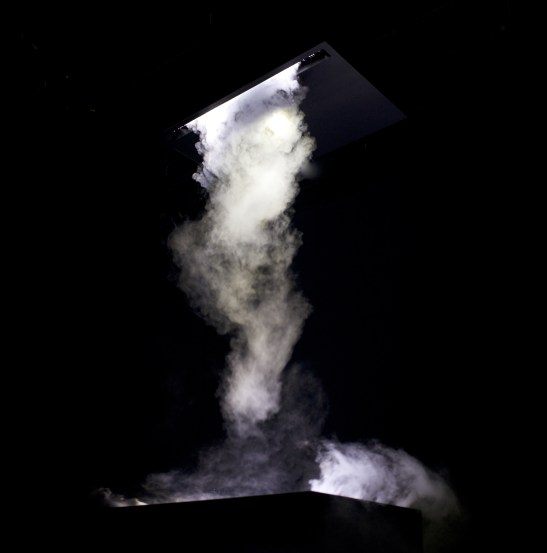
\includegraphics[width=0.6\textwidth]{images/tumbleweed.jpg}
    	\caption{Credits : Les Baltazars}
    \end{figure}
\end{frame}

\begin{frame}
    \frametitle{The software}    
    \begin{figure}
    	\centering
    	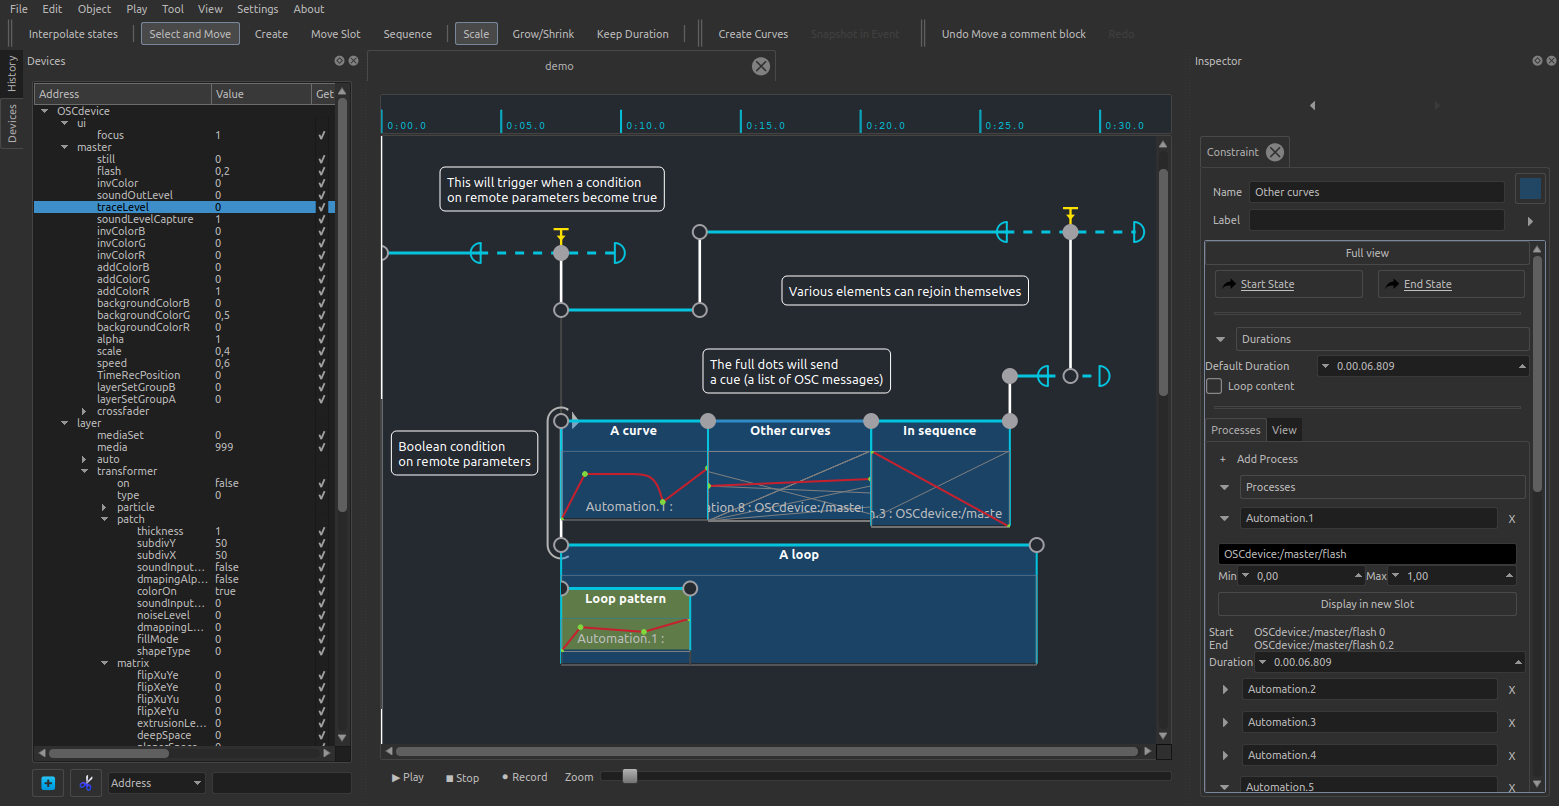
\includegraphics[width=\textwidth]{images/iscore.png}
    \end{figure}    
\end{frame}


\begin{frame}
    \frametitle{Contributors, Companies, Agencies involved}
    \begin{figure}[htbp]
    \begin{subfigure}[b]{0.30\textwidth} 
        \centering
        
\begin{tikzpicture}[scale=.05]

\pgfmathsetmacro\bleulabriR{0/255}
\pgfmathsetmacro\bleulabriG{114/255}
\pgfmathsetmacro\bleulabriB{185/255}

\pgfmathsetmacro\vertlabriR{10/255}
\pgfmathsetmacro\vertlabriG{177/255}
\pgfmathsetmacro\vertlabriB{134/255}

\pgfmathsetmacro\rougelabritopR{162/255}
\pgfmathsetmacro\rougelabritopG{47/255}
\pgfmathsetmacro\rougelabritopB{50/255}

\pgfmathsetmacro\rougelabrimiddleR{178/255}
\pgfmathsetmacro\rougelabrimiddleG{117/255}
\pgfmathsetmacro\rougelabrimiddleB{99/255}

\pgfmathsetmacro\rougelabribottomR{230/255}
\pgfmathsetmacro\rougelabribottomG{206/255}
\pgfmathsetmacro\rougelabribottomB{196/255}


\definecolor{bleulabri}{rgb}{\bleulabriR, \bleulabriG, \bleulabriB}
\definecolor{vertlabri}{rgb}{\vertlabriR, \vertlabriG, \vertlabriB}
\definecolor{rougetoplabri}{rgb}{\rougelabritopR, \rougelabritopG,
 \rougelabritopB}
\definecolor{rougemiddlelabri}{rgb}{\rougelabrimiddleR,
 \rougelabrimiddleG, \rougelabrimiddleB}
\definecolor{rougebottomlabri}{rgb}{\rougelabribottomR,
 \rougelabribottomG, \rougelabribottomB}

\def\rectanglepath{-- ++(0cm,38.5cm)-- ++(10cm,0cm)--
 ++(0cm,-30.3cm)-- ++(13cm,0cm)-- ++(-2cm,-8.2cm)-- cycle}


\shade[top color=rougetoplabri!95!black,bottom
 color=rougebottomlabri!15!white!95!black,middle
 color=rougemiddlelabri!90!white!98!black,shading=axis,
shading angle=-135] (19.25, 19.25) circle (6.75cm);

\fill[fill=bleulabri] (0,0) \rectanglepath;
\fill[rotate=180,fill=vertlabri] (-38.5,-38.5) \rectanglepath;

\end{tikzpicture}

        \caption{LaBRI \\ \url{www.labri.fr}}
    \end{subfigure}
    ~
    \begin{subfigure}[b]{0.30\textwidth} 
        \centering
        
\includegraphics[scale=0.12]{images/by.png}
        \caption[]{Blue Yeti\\ \url{www.blueyeti.fr}}
    \end{subfigure}
    ~
    \begin{subfigure}[b]{0.30\textwidth} 
        \centering
        
\includegraphics[scale=0.15]{images/gmea.png}
        \caption[]{GMEA\\\url{www.gmea.net}}
    \end{subfigure}
    
    
    \begin{subfigure}[b]{0.30\textwidth} 
        \centering
        
\includegraphics[scale=0.25]{images/cnam.png}
        \caption[]{CNAM : \\ CEDRIC, ENJMIN\\ \url{cedric.cnam.fr}}
    \end{subfigure}
    ~
    \begin{subfigure}[b]{0.30\textwidth} 
        \centering
        
\includegraphics[scale=0.05]{images/ists.jpg}
        \caption[]{ISTS\\ \url{ists-avignon.com}}
    \end{subfigure}
    ~
    \begin{subfigure}[b]{0.30\textwidth} 
        \centering
        
\includegraphics[scale=0.23]{images/ensatt.jpg}
        \caption[]{ENSATT\\ \url{ensatt.fr}}
    \end{subfigure}    
\end{figure} 
    
    {\large Artists: Les Baltazars, Renaud Rubiano, Antoine Villeret...}
    
\end{frame}

    \begin{frame}
        \frametitle{What i-score is : }
        \Large
        \begin{itemize}        
        \item<1-> A visual \textbf{programming language} \\ $\rightarrow$ Conditions, loops, structuring, in a timeline
        \item<1-> Free software : \textbf{GPL v3 }(UI) \& LGPL v2.1 (Engine)
        \item<2-> Built in \textbf{C++} (Qt, CMake)        
        \item<2-> Available on Linux / OS X / Windows        
        \item<3-> Alpha-quality \DejaSans{☹}
        \end{itemize}
    \end{frame}
    \begin{frame}
        \frametitle{What i-score is not : }
        \Large
        \begin{itemize} [<+->]
            \item PureData (yet)
            \item Ableton Live (yet)       
            \item Bug-free (yet ! \DejaSans{☺})
        \end{itemize}
        \vspace{2em}
        
        \pause[\thebeamerpauses]
        \Huge Does not operate on its own !
        \Large
        \begin{itemize} 
            \item  It's a control center
        \end{itemize}
    \end{frame}
    
    \begin{frame}
    	\centering \Huge Demonstration
    \end{frame}
    
    \begin{frame}
        \frametitle{Inter-operability}
        \Large
        \begin{itemize}
        	\item Compatible environments :\\
	        	 Max/MSP, \textbf{PureData}, Unity3D, \textbf{OpenFrameworks}, \textbf{Processing}, \textbf{Jamoma}, Modul8, Millumin, Quartz Composer, \textbf{Qt}... 
	        \item Anything that communicates over \textbf{OSC}.
	        \item Extensibilty via \textbf{plug-ins}*. \\ {\small *API not stable until v 2.0}
        \end{itemize}
        
    \end{frame}
    
    
    \begin{frame}
        \frametitle{Conditions}
        \begin{figure}
            \centering\psscalebox{0.8}{
            %LaTeX with PSTricks extensions
%%Creator: inkscape 0.91
%%Please note this file requires PSTricks extensions
\psset{xunit=.5pt,yunit=.5pt,runit=.5pt}
\begin{pspicture}(744.09448819,1052.36220472)
{
\newrgbcolor{curcolor}{0.56862748 0.48627451 0.43529412}
\pscustom[linestyle=none,fillstyle=solid,fillcolor=curcolor]
{
\newpath
\moveto(413.9,957.89280472)
\lineto(415.9,957.89280472)
\lineto(415.9,589.89280472)
\lineto(413.9,589.89280472)
\closepath
}
}
{
\newrgbcolor{curcolor}{0.36470589 0.47843137 0.21568628}
\pscustom[linestyle=none,fillstyle=solid,fillcolor=curcolor,opacity=0]
{
\newpath
\moveto(421.4,969.39280472)
\lineto(421.6516,969.58579472)
\curveto(419.6656,970.73503172)(417.3596,971.39280472)(414.9,971.39280472)
\curveto(407.44416,971.39280472)(401.4,965.34864472)(401.4,957.89280472)
\lineto(401.4,865.89280472)
\curveto(401.4,858.43680472)(407.44416,852.39280472)(414.9,852.39280472)
\curveto(417.3599,852.39280472)(419.6662,853.05080472)(421.6524,854.19980472)
}
}
{
\newrgbcolor{curcolor}{0.43921569 0.85490197 0.21176471}
\pscustom[linewidth=2,linecolor=curcolor]
{
\newpath
\moveto(421.4,969.39280472)
\lineto(421.6516,969.58579472)
\curveto(419.6656,970.73503172)(417.3596,971.39280472)(414.9,971.39280472)
\curveto(407.44416,971.39280472)(401.4,965.34864472)(401.4,957.89280472)
\lineto(401.4,865.89280472)
\curveto(401.4,858.43680472)(407.44416,852.39280472)(414.9,852.39280472)
\curveto(417.3599,852.39280472)(419.6662,853.05080472)(421.6524,854.19980472)
}
}
{
\newrgbcolor{curcolor}{1 1 1}
\pscustom[linestyle=none,fillstyle=solid,fillcolor=curcolor]
{
\newpath
\moveto(426.4,966.39280472)
\lineto(426.4,950.39280472)
\lineto(433.4,957.39280472)
}
}
{
\newrgbcolor{curcolor}{1 1 1}
\pscustom[linewidth=1,linecolor=curcolor]
{
\newpath
\moveto(426.4,966.39280472)
\lineto(426.4,950.39280472)
\lineto(433.4,957.39280472)
}
}
{
\newrgbcolor{curcolor}{1 1 1}
\pscustom[linestyle=none,fillstyle=solid,fillcolor=curcolor]
{
\newpath
\moveto(413.60000005,957.89280472)
\lineto(416.19999995,957.89280472)
\lineto(416.19999995,865.89280472)
\lineto(413.60000005,865.89280472)
\closepath
}
}
{
\newrgbcolor{curcolor}{0.43921569 0.85490197 0.21176471}
\pscustom[linewidth=1,linecolor=curcolor]
{
\newpath
\moveto(413.60000005,957.89280472)
\lineto(416.19999995,957.89280472)
\lineto(416.19999995,865.89280472)
\lineto(413.60000005,865.89280472)
\closepath
}
}
{
\newrgbcolor{curcolor}{0.36470589 0.47843137 0.21568628}
\pscustom[linestyle=none,fillstyle=solid,fillcolor=curcolor,opacity=0]
{
\newpath
\moveto(421.4,749.39280472)
\lineto(421.6516,749.58579472)
\curveto(419.6656,750.73503172)(417.3596,751.39280472)(414.9,751.39280472)
\curveto(407.44416,751.39280472)(401.4,745.34864472)(401.4,737.89280472)
\lineto(401.4,589.89280472)
\curveto(401.4,582.43680472)(407.44416,576.39280472)(414.9,576.39280472)
\curveto(417.3599,576.39280472)(419.6662,577.05080472)(421.6524,578.19980472)
}
}
{
\newrgbcolor{curcolor}{0.85490197 0.37254903 0.21176471}
\pscustom[linewidth=2,linecolor=curcolor]
{
\newpath
\moveto(421.4,749.39280472)
\lineto(421.6516,749.58579472)
\curveto(419.6656,750.73503172)(417.3596,751.39280472)(414.9,751.39280472)
\curveto(407.44416,751.39280472)(401.4,745.34864472)(401.4,737.89280472)
\lineto(401.4,589.89280472)
\curveto(401.4,582.43680472)(407.44416,576.39280472)(414.9,576.39280472)
\curveto(417.3599,576.39280472)(419.6662,577.05080472)(421.6524,578.19980472)
}
}
{
\newrgbcolor{curcolor}{1 1 1}
\pscustom[linestyle=none,fillstyle=solid,fillcolor=curcolor]
{
\newpath
\moveto(426.4,746.39280472)
\lineto(426.4,730.39280472)
\lineto(433.4,737.39280472)
}
}
{
\newrgbcolor{curcolor}{1 1 1}
\pscustom[linewidth=1,linecolor=curcolor]
{
\newpath
\moveto(426.4,746.39280472)
\lineto(426.4,730.39280472)
\lineto(433.4,737.39280472)
}
}
{
\newrgbcolor{curcolor}{1 1 1}
\pscustom[linestyle=none,fillstyle=solid,fillcolor=curcolor]
{
\newpath
\moveto(413.60000005,737.89280472)
\lineto(416.19999995,737.89280472)
\lineto(416.19999995,589.89280472)
\lineto(413.60000005,589.89280472)
\closepath
}
}
{
\newrgbcolor{curcolor}{0.85490197 0.37254903 0.21176471}
\pscustom[linewidth=1,linecolor=curcolor]
{
\newpath
\moveto(413.60000005,737.89280472)
\lineto(416.19999995,737.89280472)
\lineto(416.19999995,589.89280472)
\lineto(413.60000005,589.89280472)
\closepath
}
}
{
\newrgbcolor{curcolor}{0.01176471 0.7647059 0.86666667}
\pscustom[linewidth=3,linecolor=curcolor]
{
\newpath
\moveto(34.615,957.89280472)
\lineto(414.9,957.89280472)
}
}
{
\newrgbcolor{curcolor}{0.01176471 0.7647059 0.86666667}
\pscustom[linewidth=3,linecolor=curcolor]
{
\newpath
\moveto(414.9,865.89280472)
\lineto(569.319,865.89280472)
}
}
{
\newrgbcolor{curcolor}{0.01176471 0.7647059 0.86666667}
\pscustom[linewidth=3,linecolor=curcolor]
{
\newpath
\moveto(414.9,737.89280472)
\lineto(668.424,737.89280472)
}
}
{
\newrgbcolor{curcolor}{0.01176471 0.7647059 0.86666667}
\pscustom[linewidth=3,linecolor=curcolor]
{
\newpath
\moveto(414.9,656.89280472)
\lineto(631.547,656.89280472)
}
}
{
\newrgbcolor{curcolor}{0.14509805 0.16078432 0.1882353}
\pscustom[linestyle=none,fillstyle=solid,fillcolor=curcolor]
{
\newpath
\moveto(41.615,957.89280472)
\curveto(41.615,954.02681148)(38.48099325,950.89280472)(34.615,950.89280472)
\curveto(30.74900675,950.89280472)(27.615,954.02681148)(27.615,957.89280472)
\curveto(27.615,961.75879797)(30.74900675,964.89280472)(34.615,964.89280472)
\curveto(38.48099325,964.89280472)(41.615,961.75879797)(41.615,957.89280472)
\closepath
}
}
{
\newrgbcolor{curcolor}{0.627451 0.627451 0.64313728}
\pscustom[linewidth=2,linecolor=curcolor]
{
\newpath
\moveto(41.615,957.89280472)
\curveto(41.615,954.02681148)(38.48099325,950.89280472)(34.615,950.89280472)
\curveto(30.74900675,950.89280472)(27.615,954.02681148)(27.615,957.89280472)
\curveto(27.615,961.75879797)(30.74900675,964.89280472)(34.615,964.89280472)
\curveto(38.48099325,964.89280472)(41.615,961.75879797)(41.615,957.89280472)
\closepath
}
}
{
\newrgbcolor{curcolor}{0.14509805 0.16078432 0.1882353}
\pscustom[linestyle=none,fillstyle=solid,fillcolor=curcolor]
{
\newpath
\moveto(421.9,957.89280472)
\curveto(421.9,954.02681148)(418.76599325,950.89280472)(414.9,950.89280472)
\curveto(411.03400675,950.89280472)(407.9,954.02681148)(407.9,957.89280472)
\curveto(407.9,961.75879797)(411.03400675,964.89280472)(414.9,964.89280472)
\curveto(418.76599325,964.89280472)(421.9,961.75879797)(421.9,957.89280472)
\closepath
}
}
{
\newrgbcolor{curcolor}{0.627451 0.627451 0.64313728}
\pscustom[linewidth=2,linecolor=curcolor]
{
\newpath
\moveto(421.9,957.89280472)
\curveto(421.9,954.02681148)(418.76599325,950.89280472)(414.9,950.89280472)
\curveto(411.03400675,950.89280472)(407.9,954.02681148)(407.9,957.89280472)
\curveto(407.9,961.75879797)(411.03400675,964.89280472)(414.9,964.89280472)
\curveto(418.76599325,964.89280472)(421.9,961.75879797)(421.9,957.89280472)
\closepath
}
}
{
\newrgbcolor{curcolor}{0.14509805 0.16078432 0.1882353}
\pscustom[linestyle=none,fillstyle=solid,fillcolor=curcolor]
{
\newpath
\moveto(421.9,865.89280472)
\curveto(421.9,862.02681148)(418.76599325,858.89280472)(414.9,858.89280472)
\curveto(411.03400675,858.89280472)(407.9,862.02681148)(407.9,865.89280472)
\curveto(407.9,869.75879797)(411.03400675,872.89280472)(414.9,872.89280472)
\curveto(418.76599325,872.89280472)(421.9,869.75879797)(421.9,865.89280472)
\closepath
}
}
{
\newrgbcolor{curcolor}{0.627451 0.627451 0.64313728}
\pscustom[linewidth=2,linecolor=curcolor]
{
\newpath
\moveto(421.9,865.89280472)
\curveto(421.9,862.02681148)(418.76599325,858.89280472)(414.9,858.89280472)
\curveto(411.03400675,858.89280472)(407.9,862.02681148)(407.9,865.89280472)
\curveto(407.9,869.75879797)(411.03400675,872.89280472)(414.9,872.89280472)
\curveto(418.76599325,872.89280472)(421.9,869.75879797)(421.9,865.89280472)
\closepath
}
}
{
\newrgbcolor{curcolor}{0.14509805 0.16078432 0.1882353}
\pscustom[linestyle=none,fillstyle=solid,fillcolor=curcolor]
{
\newpath
\moveto(576.318997,865.89280472)
\curveto(576.318997,862.02681148)(573.18499025,858.89280472)(569.318997,858.89280472)
\curveto(565.45300375,858.89280472)(562.318997,862.02681148)(562.318997,865.89280472)
\curveto(562.318997,869.75879797)(565.45300375,872.89280472)(569.318997,872.89280472)
\curveto(573.18499025,872.89280472)(576.318997,869.75879797)(576.318997,865.89280472)
\closepath
}
}
{
\newrgbcolor{curcolor}{0.627451 0.627451 0.64313728}
\pscustom[linewidth=2,linecolor=curcolor]
{
\newpath
\moveto(576.318997,865.89280472)
\curveto(576.318997,862.02681148)(573.18499025,858.89280472)(569.318997,858.89280472)
\curveto(565.45300375,858.89280472)(562.318997,862.02681148)(562.318997,865.89280472)
\curveto(562.318997,869.75879797)(565.45300375,872.89280472)(569.318997,872.89280472)
\curveto(573.18499025,872.89280472)(576.318997,869.75879797)(576.318997,865.89280472)
\closepath
}
}
{
\newrgbcolor{curcolor}{0.14509805 0.16078432 0.1882353}
\pscustom[linestyle=none,fillstyle=solid,fillcolor=curcolor]
{
\newpath
\moveto(421.9,737.89280472)
\curveto(421.9,734.02681148)(418.76599325,730.89280472)(414.9,730.89280472)
\curveto(411.03400675,730.89280472)(407.9,734.02681148)(407.9,737.89280472)
\curveto(407.9,741.75879797)(411.03400675,744.89280472)(414.9,744.89280472)
\curveto(418.76599325,744.89280472)(421.9,741.75879797)(421.9,737.89280472)
\closepath
}
}
{
\newrgbcolor{curcolor}{0.627451 0.627451 0.64313728}
\pscustom[linewidth=2,linecolor=curcolor]
{
\newpath
\moveto(421.9,737.89280472)
\curveto(421.9,734.02681148)(418.76599325,730.89280472)(414.9,730.89280472)
\curveto(411.03400675,730.89280472)(407.9,734.02681148)(407.9,737.89280472)
\curveto(407.9,741.75879797)(411.03400675,744.89280472)(414.9,744.89280472)
\curveto(418.76599325,744.89280472)(421.9,741.75879797)(421.9,737.89280472)
\closepath
}
}
{
\newrgbcolor{curcolor}{0.14509805 0.16078432 0.1882353}
\pscustom[linestyle=none,fillstyle=solid,fillcolor=curcolor]
{
\newpath
\moveto(675.423997,737.89280472)
\curveto(675.423997,734.02681148)(672.28999025,730.89280472)(668.423997,730.89280472)
\curveto(664.55800375,730.89280472)(661.423997,734.02681148)(661.423997,737.89280472)
\curveto(661.423997,741.75879797)(664.55800375,744.89280472)(668.423997,744.89280472)
\curveto(672.28999025,744.89280472)(675.423997,741.75879797)(675.423997,737.89280472)
\closepath
}
}
{
\newrgbcolor{curcolor}{0.627451 0.627451 0.64313728}
\pscustom[linewidth=2,linecolor=curcolor]
{
\newpath
\moveto(675.423997,737.89280472)
\curveto(675.423997,734.02681148)(672.28999025,730.89280472)(668.423997,730.89280472)
\curveto(664.55800375,730.89280472)(661.423997,734.02681148)(661.423997,737.89280472)
\curveto(661.423997,741.75879797)(664.55800375,744.89280472)(668.423997,744.89280472)
\curveto(672.28999025,744.89280472)(675.423997,741.75879797)(675.423997,737.89280472)
\closepath
}
}
{
\newrgbcolor{curcolor}{0.14509805 0.16078432 0.1882353}
\pscustom[linestyle=none,fillstyle=solid,fillcolor=curcolor]
{
\newpath
\moveto(421.9,656.89280472)
\curveto(421.9,653.02681148)(418.76599325,649.89280472)(414.9,649.89280472)
\curveto(411.03400675,649.89280472)(407.9,653.02681148)(407.9,656.89280472)
\curveto(407.9,660.75879797)(411.03400675,663.89280472)(414.9,663.89280472)
\curveto(418.76599325,663.89280472)(421.9,660.75879797)(421.9,656.89280472)
\closepath
}
}
{
\newrgbcolor{curcolor}{0.627451 0.627451 0.64313728}
\pscustom[linewidth=2,linecolor=curcolor]
{
\newpath
\moveto(421.9,656.89280472)
\curveto(421.9,653.02681148)(418.76599325,649.89280472)(414.9,649.89280472)
\curveto(411.03400675,649.89280472)(407.9,653.02681148)(407.9,656.89280472)
\curveto(407.9,660.75879797)(411.03400675,663.89280472)(414.9,663.89280472)
\curveto(418.76599325,663.89280472)(421.9,660.75879797)(421.9,656.89280472)
\closepath
}
}
{
\newrgbcolor{curcolor}{0.14509805 0.16078432 0.1882353}
\pscustom[linestyle=none,fillstyle=solid,fillcolor=curcolor]
{
\newpath
\moveto(638.547997,656.89280472)
\curveto(638.547997,653.02681148)(635.41399025,649.89280472)(631.547997,649.89280472)
\curveto(627.68200375,649.89280472)(624.547997,653.02681148)(624.547997,656.89280472)
\curveto(624.547997,660.75879797)(627.68200375,663.89280472)(631.547997,663.89280472)
\curveto(635.41399025,663.89280472)(638.547997,660.75879797)(638.547997,656.89280472)
\closepath
}
}
{
\newrgbcolor{curcolor}{0.627451 0.627451 0.64313728}
\pscustom[linewidth=2,linecolor=curcolor]
{
\newpath
\moveto(638.547997,656.89280472)
\curveto(638.547997,653.02681148)(635.41399025,649.89280472)(631.547997,649.89280472)
\curveto(627.68200375,649.89280472)(624.547997,653.02681148)(624.547997,656.89280472)
\curveto(624.547997,660.75879797)(627.68200375,663.89280472)(631.547997,663.89280472)
\curveto(635.41399025,663.89280472)(638.547997,660.75879797)(638.547997,656.89280472)
\closepath
}
}
{
\newrgbcolor{curcolor}{0.14509805 0.16078432 0.1882353}
\pscustom[linestyle=none,fillstyle=solid,fillcolor=curcolor]
{
\newpath
\moveto(421.9,589.89280472)
\curveto(421.9,586.02681148)(418.76599325,582.89280472)(414.9,582.89280472)
\curveto(411.03400675,582.89280472)(407.9,586.02681148)(407.9,589.89280472)
\curveto(407.9,593.75879797)(411.03400675,596.89280472)(414.9,596.89280472)
\curveto(418.76599325,596.89280472)(421.9,593.75879797)(421.9,589.89280472)
\closepath
}
}
{
\newrgbcolor{curcolor}{0.627451 0.627451 0.64313728}
\pscustom[linewidth=2,linecolor=curcolor]
{
\newpath
\moveto(421.9,589.89280472)
\curveto(421.9,586.02681148)(418.76599325,582.89280472)(414.9,582.89280472)
\curveto(411.03400675,582.89280472)(407.9,586.02681148)(407.9,589.89280472)
\curveto(407.9,593.75879797)(411.03400675,596.89280472)(414.9,596.89280472)
\curveto(418.76599325,596.89280472)(421.9,593.75879797)(421.9,589.89280472)
\closepath
}
}
{
\newrgbcolor{curcolor}{0 0 0}
\pscustom[linestyle=none,fillstyle=solid,fillcolor=curcolor]
{
\newpath
\moveto(186.5709901,905.5161557)
\lineto(186.5709901,913.1061557)
\curveto(186.5709901,916.2261557)(184.5909901,918.2061557)(180.6609901,918.2061557)
\curveto(179.1009901,918.2061557)(177.4209901,917.9061557)(175.4709901,917.2161557)
\lineto(176.1609901,915.2961557)
\curveto(177.7809901,915.8661557)(179.2209901,916.1061557)(180.2709901,916.1061557)
\curveto(182.6109901,916.1061557)(184.0209901,915.2661557)(184.0209901,912.9561557)
\lineto(184.0209901,911.6661557)
\lineto(181.6809901,911.6661557)
\curveto(176.9109901,911.6661557)(174.3009901,909.8361557)(174.3009901,906.5961557)
\curveto(174.3009901,903.6561557)(176.2209901,901.7361557)(179.4009901,901.7361557)
\curveto(181.4409901,901.7361557)(183.2109901,902.4861557)(184.3509901,903.9561557)
\curveto(184.7709901,902.5161557)(185.8809901,901.8861557)(187.2309901,901.7061557)
\lineto(187.8609901,903.5061557)
\curveto(186.9609901,903.7761557)(186.5709901,904.2561557)(186.5709901,905.5161557)
\closepath
\moveto(180.0309901,903.6261557)
\curveto(177.9609901,903.6261557)(177.0009901,904.6461557)(177.0009901,906.6261557)
\curveto(177.0009901,908.6661557)(178.2609901,909.9261557)(181.7409901,909.9261557)
\lineto(184.0209901,909.9261557)
\lineto(184.0209901,905.8761557)
\curveto(183.0909901,904.4661557)(181.5909901,903.6261557)(180.0309901,903.6261557)
\closepath
}
}
{
\newrgbcolor{curcolor}{0 0 0}
\pscustom[linestyle=none,fillstyle=solid,fillcolor=curcolor]
{
\newpath
\moveto(196.78927135,914.9961557)
\curveto(196.78927135,913.6461557)(197.80927135,912.5361557)(199.18927135,912.5361557)
\curveto(200.59927135,912.5361557)(201.61927135,913.6461557)(201.61927135,914.9961557)
\curveto(201.61927135,916.3161557)(200.59927135,917.3961557)(199.18927135,917.3961557)
\curveto(197.80927135,917.3961557)(196.78927135,916.3161557)(196.78927135,914.9961557)
\closepath
\moveto(196.78927135,904.1661557)
\curveto(196.78927135,902.7861557)(197.80927135,901.7361557)(199.18927135,901.7361557)
\curveto(200.59927135,901.7361557)(201.61927135,902.7861557)(201.61927135,904.1661557)
\curveto(201.61927135,905.4861557)(200.59927135,906.5961557)(199.18927135,906.5961557)
\curveto(197.80927135,906.5961557)(196.78927135,905.4861557)(196.78927135,904.1661557)
\closepath
}
}
{
\newrgbcolor{curcolor}{0 0 0}
\pscustom[linestyle=none,fillstyle=solid,fillcolor=curcolor]
{
\newpath
\moveto(211.8375526,898.9761557)
\lineto(224.6175526,925.3761557)
\lineto(222.6075526,926.3361557)
\lineto(209.7975526,899.8761557)
\lineto(211.8375526,898.9761557)
\closepath
}
}
{
\newrgbcolor{curcolor}{0 0 0}
\pscustom[linestyle=none,fillstyle=solid,fillcolor=curcolor]
{
\newpath
\moveto(238.52583385,924.5361557)
\curveto(235.25583385,924.5361557)(232.76583385,922.7061557)(232.76583385,919.7961557)
\lineto(232.76583385,916.6461557)
\lineto(229.01583385,916.6461557)
\lineto(229.01583385,914.6361557)
\lineto(232.76583385,914.6361557)
\lineto(232.76583385,902.0661557)
\lineto(235.31583385,902.0661557)
\lineto(235.31583385,914.6361557)
\lineto(240.38583385,914.6361557)
\lineto(240.65583385,916.6461557)
\lineto(235.31583385,916.6461557)
\lineto(235.31583385,919.8561557)
\curveto(235.31583385,921.5961557)(236.42583385,922.4661557)(238.61583385,922.4661557)
\curveto(239.81583385,922.4661557)(240.98583385,922.2561557)(242.00583385,921.8061557)
\lineto(242.81583385,923.6961557)
\curveto(241.58583385,924.2061557)(240.23583385,924.5361557)(238.52583385,924.5361557)
\closepath
}
}
{
\newrgbcolor{curcolor}{0 0 0}
\pscustom[linestyle=none,fillstyle=solid,fillcolor=curcolor]
{
\newpath
\moveto(253.2141151,918.2061557)
\curveto(248.7741151,918.2061557)(246.3741151,914.8161557)(246.3741151,909.9561557)
\curveto(246.3741151,904.9761557)(248.7441151,901.7361557)(253.1841151,901.7361557)
\curveto(257.5941151,901.7361557)(259.9941151,905.1261557)(259.9941151,909.9861557)
\curveto(259.9941151,914.9661557)(257.6541151,918.2061557)(253.2141151,918.2061557)
\closepath
\moveto(253.2141151,916.1361557)
\curveto(255.9141151,916.1361557)(257.2641151,914.1561557)(257.2641151,909.9861557)
\curveto(257.2641151,905.7561557)(255.9141151,903.8061557)(253.1841151,903.8061557)
\curveto(250.4541151,903.8061557)(249.1041151,905.7561557)(249.1041151,909.9561557)
\curveto(249.1041151,914.1561557)(250.4841151,916.1361557)(253.2141151,916.1361557)
\closepath
}
}
{
\newrgbcolor{curcolor}{0 0 0}
\pscustom[linestyle=none,fillstyle=solid,fillcolor=curcolor]
{
\newpath
\moveto(271.20239635,918.2061557)
\curveto(266.76239635,918.2061557)(264.36239635,914.8161557)(264.36239635,909.9561557)
\curveto(264.36239635,904.9761557)(266.73239635,901.7361557)(271.17239635,901.7361557)
\curveto(275.58239635,901.7361557)(277.98239635,905.1261557)(277.98239635,909.9861557)
\curveto(277.98239635,914.9661557)(275.64239635,918.2061557)(271.20239635,918.2061557)
\closepath
\moveto(271.20239635,916.1361557)
\curveto(273.90239635,916.1361557)(275.25239635,914.1561557)(275.25239635,909.9861557)
\curveto(275.25239635,905.7561557)(273.90239635,903.8061557)(271.17239635,903.8061557)
\curveto(268.44239635,903.8061557)(267.09239635,905.7561557)(267.09239635,909.9561557)
\curveto(267.09239635,914.1561557)(268.47239635,916.1361557)(271.20239635,916.1361557)
\closepath
}
}
{
\newrgbcolor{curcolor}{0 0 0}
\pscustom[linestyle=none,fillstyle=solid,fillcolor=curcolor]
{
\newpath
\moveto(312.30895885,919.8861557)
\lineto(300.78895885,912.7761557)
\lineto(300.78895885,910.1661557)
\lineto(312.18895885,903.0561557)
\lineto(313.53895885,904.8861557)
\lineto(302.94895885,911.4561557)
\lineto(313.53895885,917.9661557)
\lineto(312.30895885,919.8861557)
\closepath
}
}
{
\newrgbcolor{curcolor}{0 0 0}
\pscustom[linestyle=none,fillstyle=solid,fillcolor=curcolor]
{
\newpath
\moveto(342.19552135,923.0661557)
\curveto(339.40552135,923.0661557)(337.51552135,922.0761557)(335.89552135,920.0961557)
\lineto(337.63552135,918.7461557)
\curveto(338.95552135,920.2761557)(340.06552135,920.9361557)(342.07552135,920.9361557)
\curveto(344.38552135,920.9361557)(345.79552135,919.5261557)(345.79552135,917.2161557)
\curveto(345.79552135,913.8561557)(344.11552135,911.5761557)(336.31552135,904.1061557)
\lineto(336.31552135,902.0661557)
\lineto(348.61552135,902.0661557)
\lineto(348.91552135,904.2261557)
\lineto(339.19552135,904.2261557)
\curveto(346.00552135,910.4361557)(348.43552135,913.4961557)(348.43552135,917.3061557)
\curveto(348.43552135,920.5761557)(346.09552135,923.0661557)(342.19552135,923.0661557)
\closepath
}
}
{
\newrgbcolor{curcolor}{0 0 0}
\pscustom[linestyle=none,fillstyle=solid,fillcolor=curcolor]
{
\newpath
\moveto(358.4438026,904.3761557)
\curveto(358.4438026,902.8761557)(359.5838026,901.7361557)(361.0838026,901.7361557)
\curveto(362.6138026,901.7361557)(363.7238026,902.8761557)(363.7238026,904.3761557)
\curveto(363.7238026,905.8461557)(362.6138026,907.0161557)(361.0838026,907.0161557)
\curveto(359.5838026,907.0161557)(358.4438026,905.8461557)(358.4438026,904.3761557)
\closepath
}
}
{
\newrgbcolor{curcolor}{0 0 0}
\pscustom[linestyle=none,fillstyle=solid,fillcolor=curcolor]
{
\newpath
\moveto(378.17208385,923.0661557)
\curveto(376.04208385,923.0661557)(374.06208385,922.3461557)(372.29208385,920.6661557)
\lineto(373.67208385,919.1361557)
\curveto(375.05208385,920.3961557)(376.28208385,921.0261557)(378.05208385,921.0261557)
\curveto(380.24208385,921.0261557)(381.95208385,919.7961557)(381.95208385,917.5461557)
\curveto(381.95208385,915.0561557)(380.03208385,913.9461557)(378.05208385,913.9461557)
\lineto(376.82208385,913.9461557)
\lineto(376.52208385,911.9361557)
\lineto(378.23208385,911.9361557)
\curveto(380.69208385,911.9361557)(382.52208385,910.9761557)(382.52208385,908.0061557)
\curveto(382.52208385,905.4261557)(380.81208385,903.8061557)(377.93208385,903.8061557)
\curveto(376.25208385,903.8061557)(374.51208385,904.4661557)(373.34208385,905.8461557)
\lineto(371.66208385,904.4661557)
\curveto(373.22208385,902.5761557)(375.68208385,901.7361557)(377.99208385,901.7361557)
\curveto(382.28208385,901.7361557)(385.16208385,904.4361557)(385.16208385,908.0061557)
\curveto(385.16208385,911.2161557)(382.88208385,912.8961557)(380.48208385,913.0761557)
\curveto(382.64208385,913.4961557)(384.50208385,915.3861557)(384.50208385,917.8761557)
\curveto(384.50208385,920.6961557)(382.07208385,923.0661557)(378.17208385,923.0661557)
\closepath
}
}
{
\newrgbcolor{curcolor}{0 0 0}
\pscustom[linestyle=none,fillstyle=solid,fillcolor=curcolor]
{
\newpath
\moveto(143.13446666,661.05924652)
\lineto(143.13446666,668.64924652)
\curveto(143.13446666,671.76924652)(141.15446666,673.74924652)(137.22446666,673.74924652)
\curveto(135.66446666,673.74924652)(133.98446666,673.44924652)(132.03446666,672.75924652)
\lineto(132.72446666,670.83924652)
\curveto(134.34446666,671.40924652)(135.78446666,671.64924652)(136.83446666,671.64924652)
\curveto(139.17446666,671.64924652)(140.58446666,670.80924652)(140.58446666,668.49924652)
\lineto(140.58446666,667.20924652)
\lineto(138.24446666,667.20924652)
\curveto(133.47446666,667.20924652)(130.86446666,665.37924652)(130.86446666,662.13924652)
\curveto(130.86446666,659.19924652)(132.78446666,657.27924652)(135.96446666,657.27924652)
\curveto(138.00446666,657.27924652)(139.77446666,658.02924652)(140.91446666,659.49924652)
\curveto(141.33446666,658.05924652)(142.44446666,657.42924652)(143.79446666,657.24924652)
\lineto(144.42446666,659.04924652)
\curveto(143.52446666,659.31924652)(143.13446666,659.79924652)(143.13446666,661.05924652)
\closepath
\moveto(136.59446666,659.16924652)
\curveto(134.52446666,659.16924652)(133.56446666,660.18924652)(133.56446666,662.16924652)
\curveto(133.56446666,664.20924652)(134.82446666,665.46924652)(138.30446666,665.46924652)
\lineto(140.58446666,665.46924652)
\lineto(140.58446666,661.41924652)
\curveto(139.65446666,660.00924652)(138.15446666,659.16924652)(136.59446666,659.16924652)
\closepath
}
}
{
\newrgbcolor{curcolor}{0 0 0}
\pscustom[linestyle=none,fillstyle=solid,fillcolor=curcolor]
{
\newpath
\moveto(153.35274791,670.53924652)
\curveto(153.35274791,669.18924652)(154.37274791,668.07924652)(155.75274791,668.07924652)
\curveto(157.16274791,668.07924652)(158.18274791,669.18924652)(158.18274791,670.53924652)
\curveto(158.18274791,671.85924652)(157.16274791,672.93924652)(155.75274791,672.93924652)
\curveto(154.37274791,672.93924652)(153.35274791,671.85924652)(153.35274791,670.53924652)
\closepath
\moveto(153.35274791,659.70924652)
\curveto(153.35274791,658.32924652)(154.37274791,657.27924652)(155.75274791,657.27924652)
\curveto(157.16274791,657.27924652)(158.18274791,658.32924652)(158.18274791,659.70924652)
\curveto(158.18274791,661.02924652)(157.16274791,662.13924652)(155.75274791,662.13924652)
\curveto(154.37274791,662.13924652)(153.35274791,661.02924652)(153.35274791,659.70924652)
\closepath
}
}
{
\newrgbcolor{curcolor}{0 0 0}
\pscustom[linestyle=none,fillstyle=solid,fillcolor=curcolor]
{
\newpath
\moveto(168.40102916,654.51924652)
\lineto(181.18102916,680.91924652)
\lineto(179.17102916,681.87924652)
\lineto(166.36102916,655.41924652)
\lineto(168.40102916,654.51924652)
\closepath
}
}
{
\newrgbcolor{curcolor}{0 0 0}
\pscustom[linestyle=none,fillstyle=solid,fillcolor=curcolor]
{
\newpath
\moveto(188.27931041,671.34924652)
\lineto(188.27931041,680.07924652)
\lineto(185.75931041,679.77924652)
\lineto(185.75931041,657.60924652)
\lineto(187.97931041,657.60924652)
\lineto(188.15931041,659.25924652)
\curveto(189.23931041,657.87924652)(190.64931041,657.27924652)(192.44931041,657.27924652)
\curveto(196.52931041,657.27924652)(198.71931041,660.72924652)(198.71931041,665.52924652)
\curveto(198.71931041,670.47924652)(197.00931041,673.74924652)(192.80931041,673.74924652)
\curveto(190.97931041,673.74924652)(189.44931041,672.87924652)(188.27931041,671.34924652)
\closepath
\moveto(191.87931041,659.31924652)
\curveto(190.40931041,659.31924652)(189.11931041,660.06924652)(188.27931041,661.35924652)
\lineto(188.27931041,669.18924652)
\curveto(189.14931041,670.44924652)(190.49931041,671.70924652)(192.23931041,671.70924652)
\curveto(194.69931041,671.70924652)(195.98931041,669.63924652)(195.98931041,665.52924652)
\curveto(195.98931041,661.32924652)(194.48931041,659.31924652)(191.87931041,659.31924652)
\closepath
}
}
{
\newrgbcolor{curcolor}{0 0 0}
\pscustom[linestyle=none,fillstyle=solid,fillcolor=curcolor]
{
\newpath
\moveto(215.08759166,661.05924652)
\lineto(215.08759166,668.64924652)
\curveto(215.08759166,671.76924652)(213.10759166,673.74924652)(209.17759166,673.74924652)
\curveto(207.61759166,673.74924652)(205.93759166,673.44924652)(203.98759166,672.75924652)
\lineto(204.67759166,670.83924652)
\curveto(206.29759166,671.40924652)(207.73759166,671.64924652)(208.78759166,671.64924652)
\curveto(211.12759166,671.64924652)(212.53759166,670.80924652)(212.53759166,668.49924652)
\lineto(212.53759166,667.20924652)
\lineto(210.19759166,667.20924652)
\curveto(205.42759166,667.20924652)(202.81759166,665.37924652)(202.81759166,662.13924652)
\curveto(202.81759166,659.19924652)(204.73759166,657.27924652)(207.91759166,657.27924652)
\curveto(209.95759166,657.27924652)(211.72759166,658.02924652)(212.86759166,659.49924652)
\curveto(213.28759166,658.05924652)(214.39759166,657.42924652)(215.74759166,657.24924652)
\lineto(216.37759166,659.04924652)
\curveto(215.47759166,659.31924652)(215.08759166,659.79924652)(215.08759166,661.05924652)
\closepath
\moveto(208.54759166,659.16924652)
\curveto(206.47759166,659.16924652)(205.51759166,660.18924652)(205.51759166,662.16924652)
\curveto(205.51759166,664.20924652)(206.77759166,665.46924652)(210.25759166,665.46924652)
\lineto(212.53759166,665.46924652)
\lineto(212.53759166,661.41924652)
\curveto(211.60759166,660.00924652)(210.10759166,659.16924652)(208.54759166,659.16924652)
\closepath
}
}
{
\newrgbcolor{curcolor}{0 0 0}
\pscustom[linestyle=none,fillstyle=solid,fillcolor=curcolor]
{
\newpath
\moveto(232.41587291,673.74924652)
\curveto(229.56587291,673.74924652)(227.94587291,672.24924652)(226.74587291,669.66924652)
\lineto(226.26587291,673.41924652)
\lineto(221.88587291,673.41924652)
\lineto(221.88587291,671.46924652)
\lineto(224.37587291,671.46924652)
\lineto(224.37587291,659.55924652)
\lineto(221.88587291,659.55924652)
\lineto(221.88587291,657.60924652)
\lineto(230.10587291,657.60924652)
\lineto(230.10587291,659.55924652)
\lineto(226.89587291,659.55924652)
\lineto(226.89587291,666.21924652)
\curveto(227.91587291,669.69924652)(229.65587291,671.43924652)(232.08587291,671.43924652)
\lineto(232.23587291,671.43924652)
\lineto(232.23587291,668.04924652)
\lineto(234.27587291,668.04924652)
\lineto(234.63587291,673.41924652)
\curveto(233.94587291,673.59924652)(233.28587291,673.74924652)(232.41587291,673.74924652)
\closepath
}
}
{
\newrgbcolor{curcolor}{0 0 0}
\pscustom[linestyle=none,fillstyle=solid,fillcolor=curcolor]
{
\newpath
\moveto(287.52071666,668.70924652)
\lineto(287.52071666,670.86924652)
\lineto(276.24071666,670.86924652)
\lineto(279.45071666,676.26924652)
\lineto(277.50071666,677.25924652)
\lineto(273.69071666,670.86924652)
\lineto(257.88071666,670.86924652)
\lineto(257.88071666,668.70924652)
\lineto(272.37071666,668.70924652)
\lineto(270.27071666,665.16924652)
\lineto(257.88071666,665.16924652)
\lineto(257.88071666,663.00924652)
\lineto(268.98071666,663.00924652)
\lineto(265.95071666,657.96924652)
\lineto(267.96071666,656.94924652)
\lineto(271.56071666,663.00924652)
\lineto(287.52071666,663.00924652)
\lineto(287.52071666,665.16924652)
\lineto(272.85071666,665.16924652)
\lineto(274.95071666,668.70924652)
\lineto(287.52071666,668.70924652)
\closepath
}
}
{
\newrgbcolor{curcolor}{0 0 0}
\pscustom[linestyle=none,fillstyle=solid,fillcolor=curcolor]
{
\newpath
\moveto(314.04727916,671.97924652)
\lineto(316.26727916,671.97924652)
\lineto(316.74727916,679.77924652)
\lineto(313.59727916,679.77924652)
\lineto(314.04727916,671.97924652)
\closepath
\moveto(319.08727916,671.97924652)
\lineto(321.30727916,671.97924652)
\lineto(321.75727916,679.77924652)
\lineto(318.60727916,679.77924652)
\lineto(319.08727916,671.97924652)
\closepath
}
}
{
\newrgbcolor{curcolor}{0 0 0}
\pscustom[linestyle=none,fillstyle=solid,fillcolor=curcolor]
{
\newpath
\moveto(332.18556041,671.34924652)
\lineto(332.18556041,680.07924652)
\lineto(329.66556041,679.77924652)
\lineto(329.66556041,657.60924652)
\lineto(331.88556041,657.60924652)
\lineto(332.06556041,659.25924652)
\curveto(333.14556041,657.87924652)(334.55556041,657.27924652)(336.35556041,657.27924652)
\curveto(340.43556041,657.27924652)(342.62556041,660.72924652)(342.62556041,665.52924652)
\curveto(342.62556041,670.47924652)(340.91556041,673.74924652)(336.71556041,673.74924652)
\curveto(334.88556041,673.74924652)(333.35556041,672.87924652)(332.18556041,671.34924652)
\closepath
\moveto(335.78556041,659.31924652)
\curveto(334.31556041,659.31924652)(333.02556041,660.06924652)(332.18556041,661.35924652)
\lineto(332.18556041,669.18924652)
\curveto(333.05556041,670.44924652)(334.40556041,671.70924652)(336.14556041,671.70924652)
\curveto(338.60556041,671.70924652)(339.89556041,669.63924652)(339.89556041,665.52924652)
\curveto(339.89556041,661.32924652)(338.39556041,659.31924652)(335.78556041,659.31924652)
\closepath
}
}
{
\newrgbcolor{curcolor}{0 0 0}
\pscustom[linestyle=none,fillstyle=solid,fillcolor=curcolor]
{
\newpath
\moveto(353.68384166,673.74924652)
\curveto(349.24384166,673.74924652)(346.84384166,670.35924652)(346.84384166,665.49924652)
\curveto(346.84384166,660.51924652)(349.21384166,657.27924652)(353.65384166,657.27924652)
\curveto(358.06384166,657.27924652)(360.46384166,660.66924652)(360.46384166,665.52924652)
\curveto(360.46384166,670.50924652)(358.12384166,673.74924652)(353.68384166,673.74924652)
\closepath
\moveto(353.68384166,671.67924652)
\curveto(356.38384166,671.67924652)(357.73384166,669.69924652)(357.73384166,665.52924652)
\curveto(357.73384166,661.29924652)(356.38384166,659.34924652)(353.65384166,659.34924652)
\curveto(350.92384166,659.34924652)(349.57384166,661.29924652)(349.57384166,665.49924652)
\curveto(349.57384166,669.69924652)(350.95384166,671.67924652)(353.68384166,671.67924652)
\closepath
}
}
{
\newrgbcolor{curcolor}{0 0 0}
\pscustom[linestyle=none,fillstyle=solid,fillcolor=curcolor]
{
\newpath
\moveto(371.67212291,673.74924652)
\curveto(367.23212291,673.74924652)(364.83212291,670.35924652)(364.83212291,665.49924652)
\curveto(364.83212291,660.51924652)(367.20212291,657.27924652)(371.64212291,657.27924652)
\curveto(376.05212291,657.27924652)(378.45212291,660.66924652)(378.45212291,665.52924652)
\curveto(378.45212291,670.50924652)(376.11212291,673.74924652)(371.67212291,673.74924652)
\closepath
\moveto(371.67212291,671.67924652)
\curveto(374.37212291,671.67924652)(375.72212291,669.69924652)(375.72212291,665.52924652)
\curveto(375.72212291,661.29924652)(374.37212291,659.34924652)(371.64212291,659.34924652)
\curveto(368.91212291,659.34924652)(367.56212291,661.29924652)(367.56212291,665.49924652)
\curveto(367.56212291,669.69924652)(368.94212291,671.67924652)(371.67212291,671.67924652)
\closepath
}
}
{
\newrgbcolor{curcolor}{0 0 0}
\pscustom[linestyle=none,fillstyle=solid,fillcolor=curcolor]
{
\newpath
\moveto(386.00040416,671.97924652)
\lineto(388.22040416,671.97924652)
\lineto(388.70040416,679.77924652)
\lineto(385.55040416,679.77924652)
\lineto(386.00040416,671.97924652)
\closepath
\moveto(391.04040416,671.97924652)
\lineto(393.26040416,671.97924652)
\lineto(393.71040416,679.77924652)
\lineto(390.56040416,679.77924652)
\lineto(391.04040416,671.97924652)
\closepath
}
}
{
\newrgbcolor{curcolor}{0 0 0}
\pscustom[linewidth=4,linecolor=curcolor]
{
\newpath
\moveto(298.50008,1008.13220472)
\curveto(325.64601,1000.55460472)(389.77702,1018.31510472)(412.14224,980.85810472)
}
}
{
\newrgbcolor{curcolor}{0 0 0}
\pscustom[linestyle=none,fillstyle=solid,fillcolor=curcolor]
{
\newpath
\moveto(409.68148269,984.97935131)
\lineto(404.19647944,986.36309238)
\lineto(414.80806042,976.39342092)
\lineto(411.06522375,990.46435457)
\lineto(409.68148269,984.97935131)
\closepath
}
}
{
\newrgbcolor{curcolor}{0 0 0}
\pscustom[linewidth=1,linecolor=curcolor]
{
\newpath
\moveto(409.68148269,984.97935131)
\lineto(404.19647944,986.36309238)
\lineto(414.80806042,976.39342092)
\lineto(411.06522375,990.46435457)
\lineto(409.68148269,984.97935131)
\closepath
}
}
{
\newrgbcolor{curcolor}{0 0 0}
\pscustom[linestyle=none,fillstyle=solid,fillcolor=curcolor]
{
\newpath
\moveto(84.39559947,1040.92414398)
\lineto(73.20559947,1040.92414398)
\lineto(73.20559947,1020.25414398)
\lineto(84.63559947,1020.25414398)
\lineto(84.63559947,1022.53414398)
\lineto(76.05559947,1022.53414398)
\lineto(76.05559947,1029.61414398)
\lineto(83.01559947,1029.61414398)
\lineto(83.01559947,1031.89414398)
\lineto(76.05559947,1031.89414398)
\lineto(76.05559947,1038.64414398)
\lineto(84.06559947,1038.64414398)
\lineto(84.39559947,1040.92414398)
\closepath
}
}
{
\newrgbcolor{curcolor}{0 0 0}
\pscustom[linestyle=none,fillstyle=solid,fillcolor=curcolor]
{
\newpath
\moveto(100.72028697,1036.06414398)
\lineto(97.81028697,1036.06414398)
\lineto(93.70028697,1022.71414398)
\lineto(89.56028697,1036.06414398)
\lineto(86.56028697,1036.06414398)
\lineto(92.02028697,1020.25414398)
\lineto(95.35028697,1020.25414398)
\lineto(100.72028697,1036.06414398)
\closepath
}
}
{
\newrgbcolor{curcolor}{0 0 0}
\pscustom[linestyle=none,fillstyle=solid,fillcolor=curcolor]
{
\newpath
\moveto(114.52591197,1023.94414398)
\lineto(114.52591197,1031.17414398)
\curveto(114.52591197,1034.47414398)(112.78591197,1036.42414398)(108.97591197,1036.42414398)
\curveto(107.20591197,1036.42414398)(105.46591197,1036.06414398)(103.51591197,1035.34414398)
\lineto(104.20591197,1033.33414398)
\curveto(105.82591197,1033.87414398)(107.29591197,1034.17414398)(108.46591197,1034.17414398)
\curveto(110.65591197,1034.17414398)(111.76591197,1033.33414398)(111.76591197,1031.05414398)
\lineto(111.76591197,1029.88414398)
\lineto(109.33591197,1029.88414398)
\curveto(104.92591197,1029.88414398)(102.37591197,1028.05414398)(102.37591197,1024.66414398)
\curveto(102.37591197,1021.84414398)(104.26591197,1019.89414398)(107.41591197,1019.89414398)
\curveto(109.33591197,1019.89414398)(111.01591197,1020.61414398)(112.12591197,1022.26414398)
\curveto(112.60591197,1020.70414398)(113.62591197,1020.07414398)(115.21591197,1019.89414398)
\lineto(115.84591197,1021.81414398)
\curveto(115.03591197,1022.11414398)(114.52591197,1022.56414398)(114.52591197,1023.94414398)
\closepath
\moveto(108.04591197,1021.96414398)
\curveto(106.24591197,1021.96414398)(105.31591197,1022.95414398)(105.31591197,1024.81414398)
\curveto(105.31591197,1026.97414398)(106.78591197,1028.05414398)(109.69591197,1028.05414398)
\lineto(111.76591197,1028.05414398)
\lineto(111.76591197,1024.42414398)
\curveto(110.86591197,1022.77414398)(109.66591197,1021.96414398)(108.04591197,1021.96414398)
\closepath
}
}
{
\newrgbcolor{curcolor}{0 0 0}
\pscustom[linestyle=none,fillstyle=solid,fillcolor=curcolor]
{
\newpath
\moveto(123.37356822,1019.89414398)
\curveto(124.18356822,1019.89414398)(124.96356822,1020.10414398)(125.56356822,1020.43414398)
\lineto(124.84356822,1022.35414398)
\curveto(124.54356822,1022.23414398)(124.21356822,1022.17414398)(123.82356822,1022.17414398)
\curveto(123.10356822,1022.17414398)(122.83356822,1022.59414398)(122.83356822,1023.43414398)
\lineto(122.83356822,1042.75414398)
\lineto(120.07356822,1042.42414398)
\lineto(120.07356822,1023.37414398)
\curveto(120.07356822,1021.12414398)(121.36356822,1019.89414398)(123.37356822,1019.89414398)
\closepath
}
}
{
\newrgbcolor{curcolor}{0 0 0}
\pscustom[linestyle=none,fillstyle=solid,fillcolor=curcolor]
{
\newpath
\moveto(140.77263072,1036.06414398)
\lineto(138.01263072,1036.06414398)
\lineto(138.01263072,1024.78414398)
\curveto(137.05263072,1023.19414398)(135.76263072,1022.05414398)(134.05263072,1022.05414398)
\curveto(132.34263072,1022.05414398)(131.62263072,1022.86414398)(131.62263072,1025.02414398)
\lineto(131.62263072,1036.06414398)
\lineto(128.86263072,1036.06414398)
\lineto(128.86263072,1024.72414398)
\curveto(128.86263072,1021.63414398)(130.51263072,1019.89414398)(133.27263072,1019.89414398)
\curveto(135.52263072,1019.89414398)(136.99263072,1020.79414398)(138.19263072,1022.71414398)
\lineto(138.40263072,1020.25414398)
\lineto(140.77263072,1020.25414398)
\lineto(140.77263072,1036.06414398)
\closepath
}
}
{
\newrgbcolor{curcolor}{0 0 0}
\pscustom[linestyle=none,fillstyle=solid,fillcolor=curcolor]
{
\newpath
\moveto(157.12356822,1023.94414398)
\lineto(157.12356822,1031.17414398)
\curveto(157.12356822,1034.47414398)(155.38356822,1036.42414398)(151.57356822,1036.42414398)
\curveto(149.80356822,1036.42414398)(148.06356822,1036.06414398)(146.11356822,1035.34414398)
\lineto(146.80356822,1033.33414398)
\curveto(148.42356822,1033.87414398)(149.89356822,1034.17414398)(151.06356822,1034.17414398)
\curveto(153.25356822,1034.17414398)(154.36356822,1033.33414398)(154.36356822,1031.05414398)
\lineto(154.36356822,1029.88414398)
\lineto(151.93356822,1029.88414398)
\curveto(147.52356822,1029.88414398)(144.97356822,1028.05414398)(144.97356822,1024.66414398)
\curveto(144.97356822,1021.84414398)(146.86356822,1019.89414398)(150.01356822,1019.89414398)
\curveto(151.93356822,1019.89414398)(153.61356822,1020.61414398)(154.72356822,1022.26414398)
\curveto(155.20356822,1020.70414398)(156.22356822,1020.07414398)(157.81356822,1019.89414398)
\lineto(158.44356822,1021.81414398)
\curveto(157.63356822,1022.11414398)(157.12356822,1022.56414398)(157.12356822,1023.94414398)
\closepath
\moveto(150.64356822,1021.96414398)
\curveto(148.84356822,1021.96414398)(147.91356822,1022.95414398)(147.91356822,1024.81414398)
\curveto(147.91356822,1026.97414398)(149.38356822,1028.05414398)(152.29356822,1028.05414398)
\lineto(154.36356822,1028.05414398)
\lineto(154.36356822,1024.42414398)
\curveto(153.46356822,1022.77414398)(152.26356822,1021.96414398)(150.64356822,1021.96414398)
\closepath
}
}
{
\newrgbcolor{curcolor}{0 0 0}
\pscustom[linestyle=none,fillstyle=solid,fillcolor=curcolor]
{
\newpath
\moveto(169.75122447,1022.86414398)
\curveto(168.97122447,1022.38414398)(168.34122447,1022.17414398)(167.65122447,1022.17414398)
\curveto(166.27122447,1022.17414398)(165.76122447,1022.92414398)(165.76122447,1024.51414398)
\lineto(165.76122447,1033.93414398)
\lineto(169.21122447,1033.93414398)
\lineto(169.51122447,1036.06414398)
\lineto(165.76122447,1036.06414398)
\lineto(165.76122447,1039.96414398)
\lineto(163.00122447,1039.63414398)
\lineto(163.00122447,1036.06414398)
\lineto(160.24122447,1036.06414398)
\lineto(160.24122447,1033.93414398)
\lineto(163.00122447,1033.93414398)
\lineto(163.00122447,1024.39414398)
\curveto(163.00122447,1021.45414398)(164.59122447,1019.89414398)(167.26122447,1019.89414398)
\curveto(168.61122447,1019.89414398)(169.75122447,1020.25414398)(170.80122447,1020.97414398)
\lineto(169.75122447,1022.86414398)
\closepath
}
}
{
\newrgbcolor{curcolor}{0 0 0}
\pscustom[linestyle=none,fillstyle=solid,fillcolor=curcolor]
{
\newpath
\moveto(185.30809947,1028.62414398)
\curveto(185.30809947,1033.45414398)(183.05809947,1036.42414398)(178.79809947,1036.42414398)
\curveto(174.71809947,1036.42414398)(172.22809947,1032.91414398)(172.22809947,1027.99414398)
\curveto(172.22809947,1022.98414398)(174.80809947,1019.89414398)(179.21809947,1019.89414398)
\curveto(181.40809947,1019.89414398)(183.17809947,1020.64414398)(184.73809947,1021.87414398)
\lineto(183.53809947,1023.52414398)
\curveto(182.15809947,1022.56414398)(180.98809947,1022.14414398)(179.42809947,1022.14414398)
\curveto(177.14809947,1022.14414398)(175.43809947,1023.55414398)(175.16809947,1027.21414398)
\lineto(185.24809947,1027.21414398)
\curveto(185.27809947,1027.57414398)(185.30809947,1028.08414398)(185.30809947,1028.62414398)
\closepath
\moveto(182.57809947,1029.25414398)
\lineto(175.16809947,1029.25414398)
\curveto(175.37809947,1032.76414398)(176.75809947,1034.23414398)(178.85809947,1034.23414398)
\curveto(181.34809947,1034.23414398)(182.57809947,1032.52414398)(182.57809947,1029.43414398)
\lineto(182.57809947,1029.25414398)
\closepath
}
}
{
\newrgbcolor{curcolor}{0 0 0}
\pscustom[linestyle=none,fillstyle=solid,fillcolor=curcolor]
{
\newpath
\moveto(199.37153697,1042.75414398)
\lineto(199.37153697,1034.47414398)
\curveto(198.32153697,1035.58414398)(196.97153697,1036.42414398)(195.11153697,1036.42414398)
\curveto(191.24153697,1036.42414398)(188.90153697,1032.91414398)(188.90153697,1028.08414398)
\curveto(188.90153697,1023.16414398)(191.03153697,1019.89414398)(194.87153697,1019.89414398)
\curveto(196.82153697,1019.89414398)(198.41153697,1020.85414398)(199.43153697,1022.44414398)
\lineto(199.70153697,1020.25414398)
\lineto(202.13153697,1020.25414398)
\lineto(202.13153697,1042.42414398)
\lineto(199.37153697,1042.75414398)
\closepath
\moveto(195.47153697,1022.08414398)
\curveto(193.19153697,1022.08414398)(191.87153697,1023.97414398)(191.87153697,1028.14414398)
\curveto(191.87153697,1032.25414398)(193.34153697,1034.23414398)(195.71153697,1034.23414398)
\curveto(197.27153697,1034.23414398)(198.38153697,1033.42414398)(199.37153697,1032.16414398)
\lineto(199.37153697,1024.42414398)
\curveto(198.32153697,1022.95414398)(197.24153697,1022.08414398)(195.47153697,1022.08414398)
\closepath
}
}
{
\newrgbcolor{curcolor}{0 0 0}
\pscustom[linestyle=none,fillstyle=solid,fillcolor=curcolor]
{
\newpath
\moveto(226.43997447,1023.94414398)
\lineto(226.43997447,1031.17414398)
\curveto(226.43997447,1034.47414398)(224.69997447,1036.42414398)(220.88997447,1036.42414398)
\curveto(219.11997447,1036.42414398)(217.37997447,1036.06414398)(215.42997447,1035.34414398)
\lineto(216.11997447,1033.33414398)
\curveto(217.73997447,1033.87414398)(219.20997447,1034.17414398)(220.37997447,1034.17414398)
\curveto(222.56997447,1034.17414398)(223.67997447,1033.33414398)(223.67997447,1031.05414398)
\lineto(223.67997447,1029.88414398)
\lineto(221.24997447,1029.88414398)
\curveto(216.83997447,1029.88414398)(214.28997447,1028.05414398)(214.28997447,1024.66414398)
\curveto(214.28997447,1021.84414398)(216.17997447,1019.89414398)(219.32997447,1019.89414398)
\curveto(221.24997447,1019.89414398)(222.92997447,1020.61414398)(224.03997447,1022.26414398)
\curveto(224.51997447,1020.70414398)(225.53997447,1020.07414398)(227.12997447,1019.89414398)
\lineto(227.75997447,1021.81414398)
\curveto(226.94997447,1022.11414398)(226.43997447,1022.56414398)(226.43997447,1023.94414398)
\closepath
\moveto(219.95997447,1021.96414398)
\curveto(218.15997447,1021.96414398)(217.22997447,1022.95414398)(217.22997447,1024.81414398)
\curveto(217.22997447,1026.97414398)(218.69997447,1028.05414398)(221.60997447,1028.05414398)
\lineto(223.67997447,1028.05414398)
\lineto(223.67997447,1024.42414398)
\curveto(222.77997447,1022.77414398)(221.57997447,1021.96414398)(219.95997447,1021.96414398)
\closepath
}
}
{
\newrgbcolor{curcolor}{0 0 0}
\pscustom[linestyle=none,fillstyle=solid,fillcolor=curcolor]
{
\newpath
\moveto(239.06763072,1022.86414398)
\curveto(238.28763072,1022.38414398)(237.65763072,1022.17414398)(236.96763072,1022.17414398)
\curveto(235.58763072,1022.17414398)(235.07763072,1022.92414398)(235.07763072,1024.51414398)
\lineto(235.07763072,1033.93414398)
\lineto(238.52763072,1033.93414398)
\lineto(238.82763072,1036.06414398)
\lineto(235.07763072,1036.06414398)
\lineto(235.07763072,1039.96414398)
\lineto(232.31763072,1039.63414398)
\lineto(232.31763072,1036.06414398)
\lineto(229.55763072,1036.06414398)
\lineto(229.55763072,1033.93414398)
\lineto(232.31763072,1033.93414398)
\lineto(232.31763072,1024.39414398)
\curveto(232.31763072,1021.45414398)(233.90763072,1019.89414398)(236.57763072,1019.89414398)
\curveto(237.92763072,1019.89414398)(239.06763072,1020.25414398)(240.11763072,1020.97414398)
\lineto(239.06763072,1022.86414398)
\closepath
}
}
{
\newrgbcolor{curcolor}{0 0 0}
\pscustom[linestyle=none,fillstyle=solid,fillcolor=curcolor]
{
\newpath
\moveto(257.87622447,1022.86414398)
\curveto(257.09622447,1022.38414398)(256.46622447,1022.17414398)(255.77622447,1022.17414398)
\curveto(254.39622447,1022.17414398)(253.88622447,1022.92414398)(253.88622447,1024.51414398)
\lineto(253.88622447,1033.93414398)
\lineto(257.33622447,1033.93414398)
\lineto(257.63622447,1036.06414398)
\lineto(253.88622447,1036.06414398)
\lineto(253.88622447,1039.96414398)
\lineto(251.12622447,1039.63414398)
\lineto(251.12622447,1036.06414398)
\lineto(248.36622447,1036.06414398)
\lineto(248.36622447,1033.93414398)
\lineto(251.12622447,1033.93414398)
\lineto(251.12622447,1024.39414398)
\curveto(251.12622447,1021.45414398)(252.71622447,1019.89414398)(255.38622447,1019.89414398)
\curveto(256.73622447,1019.89414398)(257.87622447,1020.25414398)(258.92622447,1020.97414398)
\lineto(257.87622447,1022.86414398)
\closepath
}
}
{
\newrgbcolor{curcolor}{0 0 0}
\pscustom[linestyle=none,fillstyle=solid,fillcolor=curcolor]
{
\newpath
\moveto(269.22606822,1036.42414398)
\curveto(267.24606822,1036.42414398)(265.68606822,1035.43414398)(264.54606822,1033.87414398)
\lineto(264.54606822,1042.69414398)
\lineto(261.78606822,1042.39414398)
\lineto(261.78606822,1020.25414398)
\lineto(264.54606822,1020.25414398)
\lineto(264.54606822,1031.50414398)
\curveto(265.59606822,1033.15414398)(266.82606822,1034.26414398)(268.53606822,1034.26414398)
\curveto(270.03606822,1034.26414398)(271.05606822,1033.57414398)(271.05606822,1031.20414398)
\lineto(271.05606822,1020.25414398)
\lineto(273.81606822,1020.25414398)
\lineto(273.81606822,1031.59414398)
\curveto(273.81606822,1034.56414398)(272.10606822,1036.42414398)(269.22606822,1036.42414398)
\closepath
}
}
{
\newrgbcolor{curcolor}{0 0 0}
\pscustom[linestyle=none,fillstyle=solid,fillcolor=curcolor]
{
\newpath
\moveto(280.71419322,1043.65414398)
\curveto(279.57419322,1043.65414398)(278.79419322,1042.84414398)(278.79419322,1041.76414398)
\curveto(278.79419322,1040.71414398)(279.57419322,1039.90414398)(280.71419322,1039.90414398)
\curveto(281.88419322,1039.90414398)(282.66419322,1040.71414398)(282.66419322,1041.76414398)
\curveto(282.66419322,1042.84414398)(281.88419322,1043.65414398)(280.71419322,1043.65414398)
\closepath
\moveto(282.12419322,1036.06414398)
\lineto(279.36419322,1036.06414398)
\lineto(279.36419322,1020.25414398)
\lineto(282.12419322,1020.25414398)
\lineto(282.12419322,1036.06414398)
\closepath
}
}
{
\newrgbcolor{curcolor}{0 0 0}
\pscustom[linestyle=none,fillstyle=solid,fillcolor=curcolor]
{
\newpath
\moveto(292.09169322,1036.42414398)
\curveto(288.82169322,1036.42414398)(286.39169322,1034.59414398)(286.39169322,1032.07414398)
\curveto(286.39169322,1029.85414398)(287.74169322,1028.38414398)(291.16169322,1027.48414398)
\curveto(294.22169322,1026.67414398)(295.00169322,1026.07414398)(295.00169322,1024.51414398)
\curveto(295.00169322,1023.01414398)(293.68169322,1022.11414398)(291.61169322,1022.11414398)
\curveto(289.90169322,1022.11414398)(288.43169322,1022.68414398)(287.17169322,1023.64414398)
\lineto(285.70169322,1021.96414398)
\curveto(287.08169322,1020.76414398)(289.00169322,1019.89414398)(291.67169322,1019.89414398)
\curveto(294.88169322,1019.89414398)(297.91169322,1021.39414398)(297.91169322,1024.69414398)
\curveto(297.91169322,1027.45414398)(295.99169322,1028.77414398)(292.66169322,1029.61414398)
\curveto(290.11169322,1030.27414398)(289.27169322,1030.87414398)(289.27169322,1032.16414398)
\curveto(289.27169322,1033.42414398)(290.38169322,1034.23414398)(292.18169322,1034.23414398)
\curveto(293.65169322,1034.23414398)(294.88169322,1033.78414398)(296.29169322,1032.88414398)
\lineto(297.46169322,1034.62414398)
\curveto(295.96169322,1035.76414398)(294.31169322,1036.42414398)(292.09169322,1036.42414398)
\closepath
}
}
{
\newrgbcolor{curcolor}{0 0 0}
\pscustom[linestyle=none,fillstyle=solid,fillcolor=curcolor]
{
\newpath
\moveto(317.03434947,1036.42414398)
\curveto(315.23434947,1036.42414398)(313.52434947,1035.55414398)(312.35434947,1033.93414398)
\lineto(312.14434947,1036.06414398)
\lineto(309.77434947,1036.06414398)
\lineto(309.77434947,1013.86414398)
\lineto(312.53434947,1014.19414398)
\lineto(312.53434947,1021.69414398)
\curveto(313.55434947,1020.46414398)(314.96434947,1019.89414398)(316.67434947,1019.89414398)
\curveto(320.75434947,1019.89414398)(322.88434947,1023.37414398)(322.88434947,1028.17414398)
\curveto(322.88434947,1033.15414398)(321.23434947,1036.42414398)(317.03434947,1036.42414398)
\closepath
\moveto(316.01434947,1022.14414398)
\curveto(314.57434947,1022.14414398)(313.34434947,1022.83414398)(312.53434947,1024.06414398)
\lineto(312.53434947,1031.77414398)
\curveto(313.37434947,1033.03414398)(314.66434947,1034.23414398)(316.34434947,1034.23414398)
\curveto(318.71434947,1034.23414398)(319.91434947,1032.28414398)(319.91434947,1028.17414398)
\curveto(319.91434947,1024.03414398)(318.53434947,1022.14414398)(316.01434947,1022.14414398)
\closepath
}
}
{
\newrgbcolor{curcolor}{0 0 0}
\pscustom[linestyle=none,fillstyle=solid,fillcolor=curcolor]
{
\newpath
\moveto(333.52684947,1036.42414398)
\curveto(329.02684947,1036.42414398)(326.44684947,1033.03414398)(326.44684947,1028.14414398)
\curveto(326.44684947,1023.13414398)(328.99684947,1019.89414398)(333.49684947,1019.89414398)
\curveto(337.96684947,1019.89414398)(340.54684947,1023.28414398)(340.54684947,1028.17414398)
\curveto(340.54684947,1033.18414398)(338.02684947,1036.42414398)(333.52684947,1036.42414398)
\closepath
\moveto(333.52684947,1034.20414398)
\curveto(336.13684947,1034.20414398)(337.57684947,1032.28414398)(337.57684947,1028.17414398)
\curveto(337.57684947,1024.03414398)(336.13684947,1022.11414398)(333.49684947,1022.11414398)
\curveto(330.85684947,1022.11414398)(329.41684947,1024.03414398)(329.41684947,1028.14414398)
\curveto(329.41684947,1032.28414398)(330.88684947,1034.20414398)(333.52684947,1034.20414398)
\closepath
}
}
{
\newrgbcolor{curcolor}{0 0 0}
\pscustom[linestyle=none,fillstyle=solid,fillcolor=curcolor]
{
\newpath
\moveto(346.45638072,1043.65414398)
\curveto(345.31638072,1043.65414398)(344.53638072,1042.84414398)(344.53638072,1041.76414398)
\curveto(344.53638072,1040.71414398)(345.31638072,1039.90414398)(346.45638072,1039.90414398)
\curveto(347.62638072,1039.90414398)(348.40638072,1040.71414398)(348.40638072,1041.76414398)
\curveto(348.40638072,1042.84414398)(347.62638072,1043.65414398)(346.45638072,1043.65414398)
\closepath
\moveto(347.86638072,1036.06414398)
\lineto(345.10638072,1036.06414398)
\lineto(345.10638072,1020.25414398)
\lineto(347.86638072,1020.25414398)
\lineto(347.86638072,1036.06414398)
\closepath
}
}
{
\newrgbcolor{curcolor}{0 0 0}
\pscustom[linestyle=none,fillstyle=solid,fillcolor=curcolor]
{
\newpath
\moveto(360.98388072,1036.42414398)
\curveto(358.91388072,1036.42414398)(357.23388072,1035.34414398)(356.15388072,1033.72414398)
\lineto(355.91388072,1036.06414398)
\lineto(353.54388072,1036.06414398)
\lineto(353.54388072,1020.25414398)
\lineto(356.30388072,1020.25414398)
\lineto(356.30388072,1031.47414398)
\curveto(357.35388072,1033.15414398)(358.55388072,1034.26414398)(360.32388072,1034.26414398)
\curveto(361.85388072,1034.26414398)(362.81388072,1033.57414398)(362.81388072,1031.20414398)
\lineto(362.81388072,1020.25414398)
\lineto(365.57388072,1020.25414398)
\lineto(365.57388072,1031.59414398)
\curveto(365.57388072,1034.59414398)(363.89388072,1036.42414398)(360.98388072,1036.42414398)
\closepath
}
}
{
\newrgbcolor{curcolor}{0 0 0}
\pscustom[linestyle=none,fillstyle=solid,fillcolor=curcolor]
{
\newpath
\moveto(378.05200572,1022.86414398)
\curveto(377.27200572,1022.38414398)(376.64200572,1022.17414398)(375.95200572,1022.17414398)
\curveto(374.57200572,1022.17414398)(374.06200572,1022.92414398)(374.06200572,1024.51414398)
\lineto(374.06200572,1033.93414398)
\lineto(377.51200572,1033.93414398)
\lineto(377.81200572,1036.06414398)
\lineto(374.06200572,1036.06414398)
\lineto(374.06200572,1039.96414398)
\lineto(371.30200572,1039.63414398)
\lineto(371.30200572,1036.06414398)
\lineto(368.54200572,1036.06414398)
\lineto(368.54200572,1033.93414398)
\lineto(371.30200572,1033.93414398)
\lineto(371.30200572,1024.39414398)
\curveto(371.30200572,1021.45414398)(372.89200572,1019.89414398)(375.56200572,1019.89414398)
\curveto(376.91200572,1019.89414398)(378.05200572,1020.25414398)(379.10200572,1020.97414398)
\lineto(378.05200572,1022.86414398)
\closepath
}
}
{
\newrgbcolor{curcolor}{0 0 0}
\pscustom[linestyle=none,fillstyle=solid,fillcolor=curcolor]
{
\newpath
\moveto(391.28059947,1043.65414398)
\curveto(390.14059947,1043.65414398)(389.36059947,1042.84414398)(389.36059947,1041.76414398)
\curveto(389.36059947,1040.71414398)(390.14059947,1039.90414398)(391.28059947,1039.90414398)
\curveto(392.45059947,1039.90414398)(393.23059947,1040.71414398)(393.23059947,1041.76414398)
\curveto(393.23059947,1042.84414398)(392.45059947,1043.65414398)(391.28059947,1043.65414398)
\closepath
\moveto(392.69059947,1036.06414398)
\lineto(389.93059947,1036.06414398)
\lineto(389.93059947,1020.25414398)
\lineto(392.69059947,1020.25414398)
\lineto(392.69059947,1036.06414398)
\closepath
}
}
{
\newrgbcolor{curcolor}{0 0 0}
\pscustom[linestyle=none,fillstyle=solid,fillcolor=curcolor]
{
\newpath
\moveto(405.80809947,1036.42414398)
\curveto(403.73809947,1036.42414398)(402.05809947,1035.34414398)(400.97809947,1033.72414398)
\lineto(400.73809947,1036.06414398)
\lineto(398.36809947,1036.06414398)
\lineto(398.36809947,1020.25414398)
\lineto(401.12809947,1020.25414398)
\lineto(401.12809947,1031.47414398)
\curveto(402.17809947,1033.15414398)(403.37809947,1034.26414398)(405.14809947,1034.26414398)
\curveto(406.67809947,1034.26414398)(407.63809947,1033.57414398)(407.63809947,1031.20414398)
\lineto(407.63809947,1020.25414398)
\lineto(410.39809947,1020.25414398)
\lineto(410.39809947,1031.59414398)
\curveto(410.39809947,1034.59414398)(408.71809947,1036.42414398)(405.80809947,1036.42414398)
\closepath
}
}
{
\newrgbcolor{curcolor}{0 0 0}
\pscustom[linestyle=none,fillstyle=solid,fillcolor=curcolor]
{
\newpath
\moveto(430.84497447,1022.86414398)
\curveto(430.06497447,1022.38414398)(429.43497447,1022.17414398)(428.74497447,1022.17414398)
\curveto(427.36497447,1022.17414398)(426.85497447,1022.92414398)(426.85497447,1024.51414398)
\lineto(426.85497447,1033.93414398)
\lineto(430.30497447,1033.93414398)
\lineto(430.60497447,1036.06414398)
\lineto(426.85497447,1036.06414398)
\lineto(426.85497447,1039.96414398)
\lineto(424.09497447,1039.63414398)
\lineto(424.09497447,1036.06414398)
\lineto(421.33497447,1036.06414398)
\lineto(421.33497447,1033.93414398)
\lineto(424.09497447,1033.93414398)
\lineto(424.09497447,1024.39414398)
\curveto(424.09497447,1021.45414398)(425.68497447,1019.89414398)(428.35497447,1019.89414398)
\curveto(429.70497447,1019.89414398)(430.84497447,1020.25414398)(431.89497447,1020.97414398)
\lineto(430.84497447,1022.86414398)
\closepath
}
}
{
\newrgbcolor{curcolor}{0 0 0}
\pscustom[linestyle=none,fillstyle=solid,fillcolor=curcolor]
{
\newpath
\moveto(436.10481822,1043.65414398)
\curveto(434.96481822,1043.65414398)(434.18481822,1042.84414398)(434.18481822,1041.76414398)
\curveto(434.18481822,1040.71414398)(434.96481822,1039.90414398)(436.10481822,1039.90414398)
\curveto(437.27481822,1039.90414398)(438.05481822,1040.71414398)(438.05481822,1041.76414398)
\curveto(438.05481822,1042.84414398)(437.27481822,1043.65414398)(436.10481822,1043.65414398)
\closepath
\moveto(437.51481822,1036.06414398)
\lineto(434.75481822,1036.06414398)
\lineto(434.75481822,1020.25414398)
\lineto(437.51481822,1020.25414398)
\lineto(437.51481822,1036.06414398)
\closepath
}
}
{
\newrgbcolor{curcolor}{0 0 0}
\pscustom[linestyle=none,fillstyle=solid,fillcolor=curcolor]
{
\newpath
\moveto(459.06231822,1036.42414398)
\curveto(456.93231822,1036.42414398)(455.49231822,1035.28414398)(454.35231822,1033.57414398)
\curveto(453.75231822,1035.37414398)(452.31231822,1036.42414398)(450.36231822,1036.42414398)
\curveto(448.29231822,1036.42414398)(446.85231822,1035.34414398)(445.80231822,1033.75414398)
\lineto(445.56231822,1036.06414398)
\lineto(443.19231822,1036.06414398)
\lineto(443.19231822,1020.25414398)
\lineto(445.95231822,1020.25414398)
\lineto(445.95231822,1031.47414398)
\curveto(447.00231822,1033.15414398)(447.96231822,1034.26414398)(449.67231822,1034.26414398)
\curveto(450.87231822,1034.26414398)(451.89231822,1033.57414398)(451.89231822,1031.20414398)
\lineto(451.89231822,1020.25414398)
\lineto(454.65231822,1020.25414398)
\lineto(454.65231822,1031.47414398)
\curveto(455.73231822,1033.15414398)(456.66231822,1034.26414398)(458.37231822,1034.26414398)
\curveto(459.57231822,1034.26414398)(460.59231822,1033.57414398)(460.59231822,1031.20414398)
\lineto(460.59231822,1020.25414398)
\lineto(463.35231822,1020.25414398)
\lineto(463.35231822,1031.59414398)
\curveto(463.35231822,1034.56414398)(461.64231822,1036.42414398)(459.06231822,1036.42414398)
\closepath
}
}
{
\newrgbcolor{curcolor}{0 0 0}
\pscustom[linestyle=none,fillstyle=solid,fillcolor=curcolor]
{
\newpath
\moveto(480.85497447,1028.62414398)
\curveto(480.85497447,1033.45414398)(478.60497447,1036.42414398)(474.34497447,1036.42414398)
\curveto(470.26497447,1036.42414398)(467.77497447,1032.91414398)(467.77497447,1027.99414398)
\curveto(467.77497447,1022.98414398)(470.35497447,1019.89414398)(474.76497447,1019.89414398)
\curveto(476.95497447,1019.89414398)(478.72497447,1020.64414398)(480.28497447,1021.87414398)
\lineto(479.08497447,1023.52414398)
\curveto(477.70497447,1022.56414398)(476.53497447,1022.14414398)(474.97497447,1022.14414398)
\curveto(472.69497447,1022.14414398)(470.98497447,1023.55414398)(470.71497447,1027.21414398)
\lineto(480.79497447,1027.21414398)
\curveto(480.82497447,1027.57414398)(480.85497447,1028.08414398)(480.85497447,1028.62414398)
\closepath
\moveto(478.12497447,1029.25414398)
\lineto(470.71497447,1029.25414398)
\curveto(470.92497447,1032.76414398)(472.30497447,1034.23414398)(474.40497447,1034.23414398)
\curveto(476.89497447,1034.23414398)(478.12497447,1032.52414398)(478.12497447,1029.43414398)
\lineto(478.12497447,1029.25414398)
\closepath
}
}
\end{pspicture}
}
        \end{figure}    
    \end{frame}
    
    \begin{frame}
        \frametitle{Triggering}
        \begin{figure}
            \centering\psscalebox{0.8}{
                %LaTeX with PSTricks extensions
%%Creator: inkscape 0.91
%%Please note this file requires PSTricks extensions
\psset{xunit=.5pt,yunit=.5pt,runit=.5pt}
\begin{pspicture}(744.09448819,1052.36220472)
{
\newrgbcolor{curcolor}{0.14509805 0.16078432 0.1882353}
\pscustom[linewidth=1,linecolor=curcolor,strokeopacity=0.15686299]
{
\newpath
\moveto(-245.56764,-12.59498528)
\lineto(1005.20236,-12.59498528)
}
}
{
\newrgbcolor{curcolor}{1 0.88235295 0}
\pscustom[linestyle=none,fillstyle=solid,fillcolor=curcolor]
{
\newpath
\moveto(389.38222392,980.01760285)
\lineto(376.69013899,980.01760285)
\lineto(376.69013899,948.48101971)
\lineto(372.03022871,948.48101971)
\lineto(372.03022871,980.01760285)
\lineto(359.33517,980.01760285)
\lineto(359.33517,984.53749472)
\lineto(389.38222392,984.53749472)
\lineto(389.38222392,980.01760285)
}
}
{
\newrgbcolor{curcolor}{1 0.88235295 0}
\pscustom[linestyle=none,fillstyle=solid,fillcolor=curcolor]
{
\newpath
\moveto(383.28003126,969.25256068)
\lineto(374.35869696,958.67572852)
\lineto(365.43736266,969.25256068)
\lineto(383.28003126,969.25256068)
}
}
{
\newrgbcolor{curcolor}{0.27450982 0.27450982 0.27450982}
\pscustom[linestyle=none,fillstyle=solid,fillcolor=curcolor]
{
\newpath
\moveto(373.43236,943.69072472)
\lineto(375.43236,943.69072472)
\lineto(375.43236,673.69072472)
\lineto(373.43236,673.69072472)
\closepath
}
}
{
\newrgbcolor{curcolor}{0.48627451 0.48627451 0.48627451}
\pscustom[linestyle=none,fillstyle=solid,fillcolor=curcolor]
{
\newpath
\moveto(373.13236005,943.69072472)
\lineto(375.73235995,943.69072472)
\lineto(375.73235995,673.69072472)
\lineto(373.13236005,673.69072472)
\closepath
}
}
{
\newrgbcolor{curcolor}{0.01176471 0.7647059 0.86666667}
\pscustom[linewidth=2.28296474,linecolor=curcolor]
{
\newpath
\moveto(111.98631,943.69072472)
\lineto(204.06370449,943.69072472)
}
}
{
\newrgbcolor{curcolor}{0.01176471 0.7647059 0.86666667}
\pscustom[linewidth=3,linecolor=curcolor,linestyle=dashed,dash=6 18]
{
\newpath
\moveto(203.43236,943.69072472)
\lineto(440.43236,943.69072472)
}
}
{
\newrgbcolor{curcolor}{0.01176471 0.7647059 0.86666667}
\pscustom[linewidth=2,linecolor=curcolor]
{
\newpath
\moveto(203.43236,953.69072472)
\curveto(197.90951,953.69072472)(193.43236,949.21357472)(193.43236,943.69072472)
\curveto(193.43236,938.16787472)(197.90951,933.69072472)(203.43236,933.69072472)
\lineto(203.43236,953.69072472)
}
}
{
\newrgbcolor{curcolor}{0.01176471 0.7647059 0.86666667}
\pscustom[linewidth=2,linecolor=curcolor]
{
\newpath
\moveto(440.43236,933.69072472)
\curveto(445.95521,933.69072472)(450.43236,938.16787472)(450.43236,943.69072472)
\curveto(450.43236,949.21357472)(445.95521,953.69072472)(440.43236,953.69072472)
\lineto(440.43236,933.69072472)
}
}
{
\newrgbcolor{curcolor}{0.01176471 0.7647059 0.86666667}
\pscustom[linewidth=3,linecolor=curcolor]
{
\newpath
\moveto(44.43236,803.69072472)
\lineto(308.43236,803.69072472)
}
}
{
\newrgbcolor{curcolor}{0.01176471 0.7647059 0.86666667}
\pscustom[linewidth=3,linecolor=curcolor,linestyle=dashed,dash=6 18]
{
\newpath
\moveto(308.43236,803.69072472)
\lineto(525.43236,803.69072472)
}
}
{
\newrgbcolor{curcolor}{0.01176471 0.7647059 0.86666667}
\pscustom[linewidth=2,linecolor=curcolor]
{
\newpath
\moveto(308.43236,813.69072472)
\curveto(302.90951,813.69072472)(298.43236,809.21357472)(298.43236,803.69072472)
\curveto(298.43236,798.16787472)(302.90951,793.69072472)(308.43236,793.69072472)
\lineto(308.43236,813.69072472)
}
}
{
\newrgbcolor{curcolor}{0.01176471 0.7647059 0.86666667}
\pscustom[linewidth=2,linecolor=curcolor]
{
\newpath
\moveto(525.43236,793.69072472)
\curveto(530.95521,793.69072472)(535.43236,798.16787472)(535.43236,803.69072472)
\curveto(535.43236,809.21357472)(530.95521,813.69072472)(525.43236,813.69072472)
\lineto(525.43236,793.69072472)
}
}
{
\newrgbcolor{curcolor}{0.01176471 0.7647059 0.86666667}
\pscustom[linewidth=3,linecolor=curcolor]
{
\newpath
\moveto(374.43236,673.69072472)
\lineto(563.43236,673.69072472)
}
}
{
\newrgbcolor{curcolor}{0.14509805 0.16078432 0.1882353}
\pscustom[linestyle=none,fillstyle=solid,fillcolor=curcolor]
{
\newpath
\moveto(115.07197,943.69072472)
\curveto(115.07197,939.82473148)(111.93796325,936.69072472)(108.07197,936.69072472)
\curveto(104.20597675,936.69072472)(101.07197,939.82473148)(101.07197,943.69072472)
\curveto(101.07197,947.55671797)(104.20597675,950.69072472)(108.07197,950.69072472)
\curveto(111.93796325,950.69072472)(115.07197,947.55671797)(115.07197,943.69072472)
\closepath
}
}
{
\newrgbcolor{curcolor}{0.627451 0.627451 0.64313728}
\pscustom[linewidth=2,linecolor=curcolor]
{
\newpath
\moveto(115.07197,943.69072472)
\curveto(115.07197,939.82473148)(111.93796325,936.69072472)(108.07197,936.69072472)
\curveto(104.20597675,936.69072472)(101.07197,939.82473148)(101.07197,943.69072472)
\curveto(101.07197,947.55671797)(104.20597675,950.69072472)(108.07197,950.69072472)
\curveto(111.93796325,950.69072472)(115.07197,947.55671797)(115.07197,943.69072472)
\closepath
}
}
{
\newrgbcolor{curcolor}{0.14509805 0.16078432 0.1882353}
\pscustom[linestyle=none,fillstyle=solid,fillcolor=curcolor]
{
\newpath
\moveto(381.43236,943.69072472)
\curveto(381.43236,939.82473148)(378.29835325,936.69072472)(374.43236,936.69072472)
\curveto(370.56636675,936.69072472)(367.43236,939.82473148)(367.43236,943.69072472)
\curveto(367.43236,947.55671797)(370.56636675,950.69072472)(374.43236,950.69072472)
\curveto(378.29835325,950.69072472)(381.43236,947.55671797)(381.43236,943.69072472)
\closepath
}
}
{
\newrgbcolor{curcolor}{0.627451 0.627451 0.64313728}
\pscustom[linewidth=2,linecolor=curcolor]
{
\newpath
\moveto(381.43236,943.69072472)
\curveto(381.43236,939.82473148)(378.29835325,936.69072472)(374.43236,936.69072472)
\curveto(370.56636675,936.69072472)(367.43236,939.82473148)(367.43236,943.69072472)
\curveto(367.43236,947.55671797)(370.56636675,950.69072472)(374.43236,950.69072472)
\curveto(378.29835325,950.69072472)(381.43236,947.55671797)(381.43236,943.69072472)
\closepath
}
}
{
\newrgbcolor{curcolor}{0.14509805 0.16078432 0.1882353}
\pscustom[linestyle=none,fillstyle=solid,fillcolor=curcolor]
{
\newpath
\moveto(381.43236,803.69072472)
\curveto(381.43236,799.82473148)(378.29835325,796.69072472)(374.43236,796.69072472)
\curveto(370.56636675,796.69072472)(367.43236,799.82473148)(367.43236,803.69072472)
\curveto(367.43236,807.55671797)(370.56636675,810.69072472)(374.43236,810.69072472)
\curveto(378.29835325,810.69072472)(381.43236,807.55671797)(381.43236,803.69072472)
\closepath
}
}
{
\newrgbcolor{curcolor}{0.627451 0.627451 0.64313728}
\pscustom[linewidth=2,linecolor=curcolor]
{
\newpath
\moveto(381.43236,803.69072472)
\curveto(381.43236,799.82473148)(378.29835325,796.69072472)(374.43236,796.69072472)
\curveto(370.56636675,796.69072472)(367.43236,799.82473148)(367.43236,803.69072472)
\curveto(367.43236,807.55671797)(370.56636675,810.69072472)(374.43236,810.69072472)
\curveto(378.29835325,810.69072472)(381.43236,807.55671797)(381.43236,803.69072472)
\closepath
}
}
{
\newrgbcolor{curcolor}{0.14509805 0.16078432 0.1882353}
\pscustom[linestyle=none,fillstyle=solid,fillcolor=curcolor]
{
\newpath
\moveto(51.43236,803.69072472)
\curveto(51.43236,799.82473148)(48.29835325,796.69072472)(44.43236,796.69072472)
\curveto(40.56636675,796.69072472)(37.43236,799.82473148)(37.43236,803.69072472)
\curveto(37.43236,807.55671797)(40.56636675,810.69072472)(44.43236,810.69072472)
\curveto(48.29835325,810.69072472)(51.43236,807.55671797)(51.43236,803.69072472)
\closepath
}
}
{
\newrgbcolor{curcolor}{0.627451 0.627451 0.64313728}
\pscustom[linewidth=2,linecolor=curcolor]
{
\newpath
\moveto(51.43236,803.69072472)
\curveto(51.43236,799.82473148)(48.29835325,796.69072472)(44.43236,796.69072472)
\curveto(40.56636675,796.69072472)(37.43236,799.82473148)(37.43236,803.69072472)
\curveto(37.43236,807.55671797)(40.56636675,810.69072472)(44.43236,810.69072472)
\curveto(48.29835325,810.69072472)(51.43236,807.55671797)(51.43236,803.69072472)
\closepath
}
}
{
\newrgbcolor{curcolor}{0.14509805 0.16078432 0.1882353}
\pscustom[linestyle=none,fillstyle=solid,fillcolor=curcolor]
{
\newpath
\moveto(381.43236,673.69072472)
\curveto(381.43236,669.82473148)(378.29835325,666.69072472)(374.43236,666.69072472)
\curveto(370.56636675,666.69072472)(367.43236,669.82473148)(367.43236,673.69072472)
\curveto(367.43236,677.55671797)(370.56636675,680.69072472)(374.43236,680.69072472)
\curveto(378.29835325,680.69072472)(381.43236,677.55671797)(381.43236,673.69072472)
\closepath
}
}
{
\newrgbcolor{curcolor}{0.627451 0.627451 0.64313728}
\pscustom[linewidth=2,linecolor=curcolor]
{
\newpath
\moveto(381.43236,673.69072472)
\curveto(381.43236,669.82473148)(378.29835325,666.69072472)(374.43236,666.69072472)
\curveto(370.56636675,666.69072472)(367.43236,669.82473148)(367.43236,673.69072472)
\curveto(367.43236,677.55671797)(370.56636675,680.69072472)(374.43236,680.69072472)
\curveto(378.29835325,680.69072472)(381.43236,677.55671797)(381.43236,673.69072472)
\closepath
}
}
{
\newrgbcolor{curcolor}{0.14509805 0.16078432 0.1882353}
\pscustom[linestyle=none,fillstyle=solid,fillcolor=curcolor]
{
\newpath
\moveto(570.43236,673.69072472)
\curveto(570.43236,669.82473148)(567.29835325,666.69072472)(563.43236,666.69072472)
\curveto(559.56636675,666.69072472)(556.43236,669.82473148)(556.43236,673.69072472)
\curveto(556.43236,677.55671797)(559.56636675,680.69072472)(563.43236,680.69072472)
\curveto(567.29835325,680.69072472)(570.43236,677.55671797)(570.43236,673.69072472)
\closepath
}
}
{
\newrgbcolor{curcolor}{0.627451 0.627451 0.64313728}
\pscustom[linewidth=2,linecolor=curcolor]
{
\newpath
\moveto(570.43236,673.69072472)
\curveto(570.43236,669.82473148)(567.29835325,666.69072472)(563.43236,666.69072472)
\curveto(559.56636675,666.69072472)(556.43236,669.82473148)(556.43236,673.69072472)
\curveto(556.43236,677.55671797)(559.56636675,680.69072472)(563.43236,680.69072472)
\curveto(567.29835325,680.69072472)(570.43236,677.55671797)(570.43236,673.69072472)
\closepath
}
}
{
\newrgbcolor{curcolor}{0 0 0}
\pscustom[linestyle=none,fillstyle=solid,fillcolor=curcolor]
{
\newpath
\moveto(112.18151771,1001.53248054)
\lineto(107.58151771,1016.28248054)
\lineto(105.25651771,1016.28248054)
\lineto(111.00651771,999.05748054)
\lineto(113.25651771,999.05748054)
\lineto(119.00651771,1016.28248054)
\lineto(116.83151771,1016.28248054)
\lineto(112.18151771,1001.53248054)
\closepath
}
}
{
\newrgbcolor{curcolor}{0 0 0}
\pscustom[linestyle=none,fillstyle=solid,fillcolor=curcolor]
{
\newpath
\moveto(127.12175209,1018.38248054)
\curveto(126.22175209,1018.38248054)(125.62175209,1017.75748054)(125.62175209,1016.90748054)
\curveto(125.62175209,1016.05748054)(126.22175209,1015.43248054)(127.12175209,1015.43248054)
\curveto(128.04675209,1015.43248054)(128.67175209,1016.05748054)(128.67175209,1016.90748054)
\curveto(128.67175209,1017.75748054)(128.04675209,1018.38248054)(127.12175209,1018.38248054)
\closepath
\moveto(128.79675209,1012.23248054)
\lineto(122.77175209,1012.23248054)
\lineto(122.77175209,1010.55748054)
\lineto(126.69675209,1010.55748054)
\lineto(126.69675209,1000.73248054)
\lineto(122.64675209,1000.73248054)
\lineto(122.64675209,999.05748054)
\lineto(132.49675209,999.05748054)
\lineto(132.49675209,1000.73248054)
\lineto(128.79675209,1000.73248054)
\lineto(128.79675209,1012.23248054)
\closepath
}
}
{
\newrgbcolor{curcolor}{0 0 0}
\pscustom[linestyle=none,fillstyle=solid,fillcolor=curcolor]
{
\newpath
\moveto(145.01198646,1017.78248054)
\lineto(145.01198646,1010.93248054)
\curveto(144.11198646,1011.95748054)(142.98698646,1012.50748054)(141.46198646,1012.50748054)
\curveto(138.23698646,1012.50748054)(136.31198646,1009.58248054)(136.31198646,1005.63248054)
\curveto(136.31198646,1001.53248054)(137.88698646,998.78248054)(141.33698646,998.78248054)
\curveto(142.76198646,998.78248054)(144.08698646,999.40748054)(145.06198646,1000.78248054)
\lineto(145.26198646,999.05748054)
\lineto(147.11198646,999.05748054)
\lineto(147.11198646,1017.53248054)
\lineto(145.01198646,1017.78248054)
\closepath
\moveto(142.01198646,1010.80748054)
\curveto(143.23698646,1010.80748054)(144.28698646,1010.18248054)(145.01198646,1009.10748054)
\lineto(145.01198646,1002.55748054)
\curveto(144.28698646,1001.45748054)(143.26198646,1000.45748054)(141.76198646,1000.45748054)
\curveto(139.68698646,1000.45748054)(138.58698646,1002.20748054)(138.58698646,1005.63248054)
\curveto(138.58698646,1009.10748054)(139.83698646,1010.80748054)(142.01198646,1010.80748054)
\closepath
}
}
{
\newrgbcolor{curcolor}{0 0 0}
\pscustom[linestyle=none,fillstyle=solid,fillcolor=curcolor]
{
\newpath
\moveto(153.77722084,1004.90748054)
\lineto(162.62722084,1004.90748054)
\curveto(162.65222084,1005.18248054)(162.67722084,1005.58248054)(162.67722084,1006.03248054)
\curveto(162.67722084,1010.03248054)(160.62722084,1012.50748054)(157.30222084,1012.50748054)
\curveto(153.80222084,1012.50748054)(151.57722084,1009.60748054)(151.57722084,1005.63248054)
\curveto(151.57722084,1001.53248054)(153.75222084,998.78248054)(157.60222084,998.78248054)
\curveto(159.22722084,998.78248054)(160.87722084,999.35748054)(162.10222084,1000.30748054)
\lineto(161.12722084,1001.70748054)
\curveto(159.95222084,1000.93248054)(158.95222084,1000.53248054)(157.60222084,1000.53248054)
\curveto(155.57722084,1000.53248054)(153.87722084,1001.85748054)(153.77722084,1004.90748054)
\closepath
\moveto(157.32722084,1010.78248054)
\curveto(159.32722084,1010.78248054)(160.57722084,1009.33248054)(160.62722084,1006.50748054)
\lineto(153.77722084,1006.50748054)
\curveto(153.95222084,1009.40748054)(155.37722084,1010.78248054)(157.32722084,1010.78248054)
\closepath
}
}
{
\newrgbcolor{curcolor}{0 0 0}
\pscustom[linestyle=none,fillstyle=solid,fillcolor=curcolor]
{
\newpath
\moveto(172.11745521,1012.50748054)
\curveto(168.41745521,1012.50748054)(166.41745521,1009.68248054)(166.41745521,1005.63248054)
\curveto(166.41745521,1001.48248054)(168.39245521,998.78248054)(172.09245521,998.78248054)
\curveto(175.76745521,998.78248054)(177.76745521,1001.60748054)(177.76745521,1005.65748054)
\curveto(177.76745521,1009.80748054)(175.81745521,1012.50748054)(172.11745521,1012.50748054)
\closepath
\moveto(172.11745521,1010.78248054)
\curveto(174.36745521,1010.78248054)(175.49245521,1009.13248054)(175.49245521,1005.65748054)
\curveto(175.49245521,1002.13248054)(174.36745521,1000.50748054)(172.09245521,1000.50748054)
\curveto(169.81745521,1000.50748054)(168.69245521,1002.13248054)(168.69245521,1005.63248054)
\curveto(168.69245521,1009.13248054)(169.84245521,1010.78248054)(172.11745521,1010.78248054)
\closepath
}
}
{
\newrgbcolor{curcolor}{0 0 0}
\pscustom[linestyle=none,fillstyle=solid,fillcolor=curcolor]
{
\newpath
\moveto(185.05768959,1009.83248054)
\curveto(185.05768959,1008.70748054)(185.90768959,1007.78248054)(187.05768959,1007.78248054)
\curveto(188.23268959,1007.78248054)(189.08268959,1008.70748054)(189.08268959,1009.83248054)
\curveto(189.08268959,1010.93248054)(188.23268959,1011.83248054)(187.05768959,1011.83248054)
\curveto(185.90768959,1011.83248054)(185.05768959,1010.93248054)(185.05768959,1009.83248054)
\closepath
\moveto(185.05768959,1000.80748054)
\curveto(185.05768959,999.65748054)(185.90768959,998.78248054)(187.05768959,998.78248054)
\curveto(188.23268959,998.78248054)(189.08268959,999.65748054)(189.08268959,1000.80748054)
\curveto(189.08268959,1001.90748054)(188.23268959,1002.83248054)(187.05768959,1002.83248054)
\curveto(185.90768959,1002.83248054)(185.05768959,1001.90748054)(185.05768959,1000.80748054)
\closepath
}
}
{
\newrgbcolor{curcolor}{0 0 0}
\pscustom[linestyle=none,fillstyle=solid,fillcolor=curcolor]
{
\newpath
\moveto(197.59792396,996.48248054)
\lineto(208.24792396,1018.48248054)
\lineto(206.57292396,1019.28248054)
\lineto(195.89792396,997.23248054)
\lineto(197.59792396,996.48248054)
\closepath
}
}
{
\newrgbcolor{curcolor}{0 0 0}
\pscustom[linestyle=none,fillstyle=solid,fillcolor=curcolor]
{
\newpath
\moveto(217.96315834,1012.50748054)
\curveto(216.38815834,1012.50748054)(214.98815834,1011.73248054)(214.03815834,1010.38248054)
\lineto(213.86315834,1012.23248054)
\lineto(212.06315834,1012.23248054)
\lineto(212.06315834,993.75748054)
\lineto(214.16315834,994.00748054)
\lineto(214.16315834,1000.28248054)
\curveto(215.06315834,999.28248054)(216.21315834,998.78248054)(217.66315834,998.78248054)
\curveto(221.08815834,998.78248054)(222.73815834,1001.65748054)(222.73815834,1005.65748054)
\curveto(222.73815834,1009.78248054)(221.46315834,1012.50748054)(217.96315834,1012.50748054)
\closepath
\moveto(217.46315834,1010.80748054)
\curveto(219.53815834,1010.80748054)(220.46315834,1009.08248054)(220.46315834,1005.65748054)
\curveto(220.46315834,1002.15748054)(219.36315834,1000.53248054)(217.18815834,1000.53248054)
\curveto(215.93815834,1000.53248054)(214.86315834,1001.15748054)(214.16315834,1002.18248054)
\lineto(214.16315834,1008.70748054)
\curveto(214.88815834,1009.75748054)(216.01315834,1010.80748054)(217.46315834,1010.80748054)
\closepath
}
}
{
\newrgbcolor{curcolor}{0 0 0}
\pscustom[linestyle=none,fillstyle=solid,fillcolor=curcolor]
{
\newpath
\moveto(232.07839271,1012.50748054)
\curveto(228.37839271,1012.50748054)(226.37839271,1009.68248054)(226.37839271,1005.63248054)
\curveto(226.37839271,1001.48248054)(228.35339271,998.78248054)(232.05339271,998.78248054)
\curveto(235.72839271,998.78248054)(237.72839271,1001.60748054)(237.72839271,1005.65748054)
\curveto(237.72839271,1009.80748054)(235.77839271,1012.50748054)(232.07839271,1012.50748054)
\closepath
\moveto(232.07839271,1010.78248054)
\curveto(234.32839271,1010.78248054)(235.45339271,1009.13248054)(235.45339271,1005.65748054)
\curveto(235.45339271,1002.13248054)(234.32839271,1000.50748054)(232.05339271,1000.50748054)
\curveto(229.77839271,1000.50748054)(228.65339271,1002.13248054)(228.65339271,1005.63248054)
\curveto(228.65339271,1009.13248054)(229.80339271,1010.78248054)(232.07839271,1010.78248054)
\closepath
}
}
{
\newrgbcolor{curcolor}{0 0 0}
\pscustom[linestyle=none,fillstyle=solid,fillcolor=curcolor]
{
\newpath
\moveto(242.04362709,999.05748054)
\lineto(244.14362709,999.05748054)
\lineto(244.14362709,1008.63248054)
\curveto(244.84362709,1009.68248054)(246.16862709,1010.83248054)(247.71862709,1010.83248054)
\curveto(249.69362709,1010.83248054)(249.96862709,1009.75748054)(249.96862709,1007.05748054)
\lineto(249.96862709,999.05748054)
\lineto(252.06862709,999.05748054)
\lineto(252.06862709,1008.60748054)
\curveto(252.06862709,1011.05748054)(250.94362709,1012.50748054)(248.36862709,1012.50748054)
\curveto(246.81862709,1012.50748054)(245.06862709,1011.73248054)(244.01862709,1010.38248054)
\lineto(243.84362709,1012.23248054)
\lineto(242.04362709,1012.23248054)
\lineto(242.04362709,999.05748054)
\closepath
}
}
{
\newrgbcolor{curcolor}{0 0 0}
\pscustom[linestyle=none,fillstyle=solid,fillcolor=curcolor]
{
\newpath
\moveto(267.98386146,1012.23248054)
\lineto(265.80886146,1012.23248054)
\lineto(262.08386146,1000.65748054)
\lineto(258.30886146,1012.23248054)
\lineto(256.08386146,1012.23248054)
\lineto(260.65886146,999.05748054)
\lineto(261.35886146,999.05748054)
\curveto(260.68386146,997.03248054)(259.88386146,995.90748054)(257.18386146,995.43248054)
\lineto(257.48386146,993.75748054)
\curveto(260.98386146,994.13248054)(262.45886146,996.28248054)(263.38386146,998.98248054)
\lineto(267.98386146,1012.23248054)
\closepath
}
}
{
\newrgbcolor{curcolor}{0 0 0}
\pscustom[linestyle=none,fillstyle=solid,fillcolor=curcolor]
{
\newpath
\moveto(272.54909584,996.48248054)
\lineto(283.19909584,1018.48248054)
\lineto(281.52409584,1019.28248054)
\lineto(270.84909584,997.23248054)
\lineto(272.54909584,996.48248054)
\closepath
}
}
{
\newrgbcolor{curcolor}{0 0 0}
\pscustom[linestyle=none,fillstyle=solid,fillcolor=curcolor]
{
\newpath
\moveto(289.11433021,1010.50748054)
\lineto(289.11433021,1017.78248054)
\lineto(287.01433021,1017.53248054)
\lineto(287.01433021,999.05748054)
\lineto(288.86433021,999.05748054)
\lineto(289.01433021,1000.43248054)
\curveto(289.91433021,999.28248054)(291.08933021,998.78248054)(292.58933021,998.78248054)
\curveto(295.98933021,998.78248054)(297.81433021,1001.65748054)(297.81433021,1005.65748054)
\curveto(297.81433021,1009.78248054)(296.38933021,1012.50748054)(292.88933021,1012.50748054)
\curveto(291.36433021,1012.50748054)(290.08933021,1011.78248054)(289.11433021,1010.50748054)
\closepath
\moveto(292.11433021,1000.48248054)
\curveto(290.88933021,1000.48248054)(289.81433021,1001.10748054)(289.11433021,1002.18248054)
\lineto(289.11433021,1008.70748054)
\curveto(289.83933021,1009.75748054)(290.96433021,1010.80748054)(292.41433021,1010.80748054)
\curveto(294.46433021,1010.80748054)(295.53933021,1009.08248054)(295.53933021,1005.65748054)
\curveto(295.53933021,1002.15748054)(294.28933021,1000.48248054)(292.11433021,1000.48248054)
\closepath
}
}
{
\newrgbcolor{curcolor}{0 0 0}
\pscustom[linestyle=none,fillstyle=solid,fillcolor=curcolor]
{
\newpath
\moveto(303.67956459,1004.90748054)
\lineto(312.52956459,1004.90748054)
\curveto(312.55456459,1005.18248054)(312.57956459,1005.58248054)(312.57956459,1006.03248054)
\curveto(312.57956459,1010.03248054)(310.52956459,1012.50748054)(307.20456459,1012.50748054)
\curveto(303.70456459,1012.50748054)(301.47956459,1009.60748054)(301.47956459,1005.63248054)
\curveto(301.47956459,1001.53248054)(303.65456459,998.78248054)(307.50456459,998.78248054)
\curveto(309.12956459,998.78248054)(310.77956459,999.35748054)(312.00456459,1000.30748054)
\lineto(311.02956459,1001.70748054)
\curveto(309.85456459,1000.93248054)(308.85456459,1000.53248054)(307.50456459,1000.53248054)
\curveto(305.47956459,1000.53248054)(303.77956459,1001.85748054)(303.67956459,1004.90748054)
\closepath
\moveto(307.22956459,1010.78248054)
\curveto(309.22956459,1010.78248054)(310.47956459,1009.33248054)(310.52956459,1006.50748054)
\lineto(303.67956459,1006.50748054)
\curveto(303.85456459,1009.40748054)(305.27956459,1010.78248054)(307.22956459,1010.78248054)
\closepath
}
}
{
\newrgbcolor{curcolor}{0 0 0}
\pscustom[linestyle=none,fillstyle=solid,fillcolor=curcolor]
{
\newpath
\moveto(321.49479896,1000.50748054)
\curveto(319.94479896,1000.50748054)(318.54479896,1001.08248054)(317.51979896,1001.93248054)
\lineto(316.34479896,1000.55748054)
\curveto(317.46979896,999.58248054)(319.09479896,998.78248054)(321.49479896,998.78248054)
\curveto(324.29479896,998.78248054)(327.01979896,999.88248054)(327.01979896,1002.70748054)
\curveto(327.01979896,1005.15748054)(325.31979896,1006.05748054)(322.74479896,1006.75748054)
\curveto(320.09479896,1007.48248054)(319.26979896,1007.88248054)(319.26979896,1009.08248054)
\curveto(319.26979896,1010.08248054)(320.01979896,1010.80748054)(322.11979896,1010.80748054)
\curveto(323.81979896,1010.80748054)(324.94479896,1010.28248054)(325.91979896,1009.60748054)
\lineto(326.86979896,1011.05748054)
\curveto(325.74479896,1011.85748054)(324.19479896,1012.50748054)(322.06979896,1012.50748054)
\curveto(319.09479896,1012.50748054)(317.06979896,1011.10748054)(317.06979896,1008.90748054)
\curveto(317.06979896,1006.60748054)(318.84479896,1005.78248054)(321.56979896,1005.10748054)
\curveto(324.36979896,1004.40748054)(324.74479896,1003.78248054)(324.74479896,1002.60748054)
\curveto(324.74479896,1001.33248054)(323.51979896,1000.50748054)(321.49479896,1000.50748054)
\closepath
}
}
{
\newrgbcolor{curcolor}{0 0 0}
\pscustom[linestyle=none,fillstyle=solid,fillcolor=curcolor]
{
\newpath
\moveto(342.46003334,999.73248054)
\lineto(341.63503334,1001.15748054)
\curveto(340.93503334,1000.78248054)(340.08503334,1000.53248054)(339.11003334,1000.53248054)
\curveto(337.31003334,1000.53248054)(336.58503334,1001.30748054)(336.58503334,1002.75748054)
\lineto(336.58503334,1010.58248054)
\lineto(340.88503334,1010.58248054)
\lineto(341.16003334,1012.23248054)
\lineto(336.58503334,1012.23248054)
\lineto(336.58503334,1015.45748054)
\lineto(334.48503334,1015.20748054)
\lineto(334.48503334,1012.23248054)
\lineto(331.46003334,1012.23248054)
\lineto(331.46003334,1010.58248054)
\lineto(334.48503334,1010.58248054)
\lineto(334.48503334,1002.73248054)
\curveto(334.48503334,1000.43248054)(336.08503334,998.78248054)(338.91003334,998.78248054)
\curveto(340.16003334,998.78248054)(341.53503334,999.13248054)(342.46003334,999.73248054)
\closepath
}
}
{
\newrgbcolor{curcolor}{0 0 0}
\pscustom[linestyle=none,fillstyle=solid,fillcolor=curcolor]
{
\newpath
\moveto(386.80573646,1010.10748054)
\lineto(362.10573646,1010.10748054)
\lineto(362.10573646,1008.30748054)
\lineto(386.80573646,1008.30748054)
\lineto(386.80573646,1010.10748054)
\closepath
\moveto(386.80573646,1005.35748054)
\lineto(362.10573646,1005.35748054)
\lineto(362.10573646,1003.55748054)
\lineto(386.80573646,1003.55748054)
\lineto(386.80573646,1005.35748054)
\closepath
}
}
{
\newrgbcolor{curcolor}{0 0 0}
\pscustom[linestyle=none,fillstyle=solid,fillcolor=curcolor]
{
\newpath
\moveto(408.91120521,1011.03248054)
\lineto(410.76120521,1011.03248054)
\lineto(411.16120521,1017.53248054)
\lineto(408.53620521,1017.53248054)
\lineto(408.91120521,1011.03248054)
\closepath
\moveto(413.11120521,1011.03248054)
\lineto(414.96120521,1011.03248054)
\lineto(415.33620521,1017.53248054)
\lineto(412.71120521,1017.53248054)
\lineto(413.11120521,1011.03248054)
\closepath
}
}
{
\newrgbcolor{curcolor}{0 0 0}
\pscustom[linestyle=none,fillstyle=solid,fillcolor=curcolor]
{
\newpath
\moveto(425.05143959,1014.48248054)
\lineto(432.77643959,1014.48248054)
\lineto(433.02643959,1016.28248054)
\lineto(422.87643959,1016.28248054)
\lineto(422.87643959,999.05748054)
\lineto(425.05143959,999.05748054)
\lineto(425.05143959,1006.70748054)
\lineto(431.80143959,1006.70748054)
\lineto(431.80143959,1008.45748054)
\lineto(425.05143959,1008.45748054)
\lineto(425.05143959,1014.48248054)
\closepath
}
}
{
\newrgbcolor{curcolor}{0 0 0}
\pscustom[linestyle=none,fillstyle=solid,fillcolor=curcolor]
{
\newpath
\moveto(442.06667396,1017.53248054)
\lineto(435.91667396,1017.53248054)
\lineto(435.91667396,1015.85748054)
\lineto(439.96667396,1015.85748054)
\lineto(439.96667396,1002.40748054)
\curveto(439.96667396,1000.13248054)(441.54167396,998.78248054)(443.86667396,998.78248054)
\curveto(445.21667396,998.78248054)(446.29167396,999.08248054)(446.99167396,999.45748054)
\lineto(446.44167396,1000.98248054)
\curveto(445.71667396,1000.70748054)(445.01667396,1000.53248054)(444.24167396,1000.53248054)
\curveto(442.96667396,1000.53248054)(442.06667396,1001.00748054)(442.06667396,1002.30748054)
\lineto(442.06667396,1017.53248054)
\closepath
}
}
{
\newrgbcolor{curcolor}{0 0 0}
\pscustom[linestyle=none,fillstyle=solid,fillcolor=curcolor]
{
\newpath
\moveto(454.00690834,1012.23248054)
\lineto(451.90690834,1012.23248054)
\lineto(451.90690834,1002.65748054)
\curveto(451.90690834,1000.20748054)(453.15690834,998.78248054)(455.70690834,998.78248054)
\curveto(457.25690834,998.78248054)(458.88190834,999.50748054)(459.93190834,1000.83248054)
\lineto(460.10690834,999.05748054)
\lineto(461.90690834,999.05748054)
\lineto(461.90690834,1012.23248054)
\lineto(459.80690834,1012.23248054)
\lineto(459.80690834,1002.53248054)
\curveto(459.08190834,1001.40748054)(457.68190834,1000.43248054)(456.23190834,1000.43248054)
\curveto(454.70690834,1000.43248054)(454.00690834,1001.18248054)(454.00690834,1002.88248054)
\lineto(454.00690834,1012.23248054)
\closepath
}
}
{
\newrgbcolor{curcolor}{0 0 0}
\pscustom[linestyle=none,fillstyle=solid,fillcolor=curcolor]
{
\newpath
\moveto(477.37214271,999.73248054)
\lineto(476.54714271,1001.15748054)
\curveto(475.84714271,1000.78248054)(474.99714271,1000.53248054)(474.02214271,1000.53248054)
\curveto(472.22214271,1000.53248054)(471.49714271,1001.30748054)(471.49714271,1002.75748054)
\lineto(471.49714271,1010.58248054)
\lineto(475.79714271,1010.58248054)
\lineto(476.07214271,1012.23248054)
\lineto(471.49714271,1012.23248054)
\lineto(471.49714271,1015.45748054)
\lineto(469.39714271,1015.20748054)
\lineto(469.39714271,1012.23248054)
\lineto(466.37214271,1012.23248054)
\lineto(466.37214271,1010.58248054)
\lineto(469.39714271,1010.58248054)
\lineto(469.39714271,1002.73248054)
\curveto(469.39714271,1000.43248054)(470.99714271,998.78248054)(473.82214271,998.78248054)
\curveto(475.07214271,998.78248054)(476.44714271,999.13248054)(477.37214271,999.73248054)
\closepath
}
}
{
\newrgbcolor{curcolor}{0 0 0}
\pscustom[linestyle=none,fillstyle=solid,fillcolor=curcolor]
{
\newpath
\moveto(492.36237709,999.73248054)
\lineto(491.53737709,1001.15748054)
\curveto(490.83737709,1000.78248054)(489.98737709,1000.53248054)(489.01237709,1000.53248054)
\curveto(487.21237709,1000.53248054)(486.48737709,1001.30748054)(486.48737709,1002.75748054)
\lineto(486.48737709,1010.58248054)
\lineto(490.78737709,1010.58248054)
\lineto(491.06237709,1012.23248054)
\lineto(486.48737709,1012.23248054)
\lineto(486.48737709,1015.45748054)
\lineto(484.38737709,1015.20748054)
\lineto(484.38737709,1012.23248054)
\lineto(481.36237709,1012.23248054)
\lineto(481.36237709,1010.58248054)
\lineto(484.38737709,1010.58248054)
\lineto(484.38737709,1002.73248054)
\curveto(484.38737709,1000.43248054)(485.98737709,998.78248054)(488.81237709,998.78248054)
\curveto(490.06237709,998.78248054)(491.43737709,999.13248054)(492.36237709,999.73248054)
\closepath
}
}
{
\newrgbcolor{curcolor}{0 0 0}
\pscustom[linestyle=none,fillstyle=solid,fillcolor=curcolor]
{
\newpath
\moveto(498.55261146,1004.90748054)
\lineto(507.40261146,1004.90748054)
\curveto(507.42761146,1005.18248054)(507.45261146,1005.58248054)(507.45261146,1006.03248054)
\curveto(507.45261146,1010.03248054)(505.40261146,1012.50748054)(502.07761146,1012.50748054)
\curveto(498.57761146,1012.50748054)(496.35261146,1009.60748054)(496.35261146,1005.63248054)
\curveto(496.35261146,1001.53248054)(498.52761146,998.78248054)(502.37761146,998.78248054)
\curveto(504.00261146,998.78248054)(505.65261146,999.35748054)(506.87761146,1000.30748054)
\lineto(505.90261146,1001.70748054)
\curveto(504.72761146,1000.93248054)(503.72761146,1000.53248054)(502.37761146,1000.53248054)
\curveto(500.35261146,1000.53248054)(498.65261146,1001.85748054)(498.55261146,1004.90748054)
\closepath
\moveto(502.10261146,1010.78248054)
\curveto(504.10261146,1010.78248054)(505.35261146,1009.33248054)(505.40261146,1006.50748054)
\lineto(498.55261146,1006.50748054)
\curveto(498.72761146,1009.40748054)(500.15261146,1010.78248054)(502.10261146,1010.78248054)
\closepath
}
}
{
\newrgbcolor{curcolor}{0 0 0}
\pscustom[linestyle=none,fillstyle=solid,fillcolor=curcolor]
{
\newpath
\moveto(520.76784584,1012.50748054)
\curveto(518.39284584,1012.50748054)(517.04284584,1011.25748054)(516.04284584,1009.10748054)
\lineto(515.64284584,1012.23248054)
\lineto(511.99284584,1012.23248054)
\lineto(511.99284584,1010.60748054)
\lineto(514.06784584,1010.60748054)
\lineto(514.06784584,1000.68248054)
\lineto(511.99284584,1000.68248054)
\lineto(511.99284584,999.05748054)
\lineto(518.84284584,999.05748054)
\lineto(518.84284584,1000.68248054)
\lineto(516.16784584,1000.68248054)
\lineto(516.16784584,1006.23248054)
\curveto(517.01784584,1009.13248054)(518.46784584,1010.58248054)(520.49284584,1010.58248054)
\lineto(520.61784584,1010.58248054)
\lineto(520.61784584,1007.75748054)
\lineto(522.31784584,1007.75748054)
\lineto(522.61784584,1012.23248054)
\curveto(522.04284584,1012.38248054)(521.49284584,1012.50748054)(520.76784584,1012.50748054)
\closepath
}
}
{
\newrgbcolor{curcolor}{0 0 0}
\pscustom[linestyle=none,fillstyle=solid,fillcolor=curcolor]
{
\newpath
\moveto(531.35808021,1000.50748054)
\curveto(529.80808021,1000.50748054)(528.40808021,1001.08248054)(527.38308021,1001.93248054)
\lineto(526.20808021,1000.55748054)
\curveto(527.33308021,999.58248054)(528.95808021,998.78248054)(531.35808021,998.78248054)
\curveto(534.15808021,998.78248054)(536.88308021,999.88248054)(536.88308021,1002.70748054)
\curveto(536.88308021,1005.15748054)(535.18308021,1006.05748054)(532.60808021,1006.75748054)
\curveto(529.95808021,1007.48248054)(529.13308021,1007.88248054)(529.13308021,1009.08248054)
\curveto(529.13308021,1010.08248054)(529.88308021,1010.80748054)(531.98308021,1010.80748054)
\curveto(533.68308021,1010.80748054)(534.80808021,1010.28248054)(535.78308021,1009.60748054)
\lineto(536.73308021,1011.05748054)
\curveto(535.60808021,1011.85748054)(534.05808021,1012.50748054)(531.93308021,1012.50748054)
\curveto(528.95808021,1012.50748054)(526.93308021,1011.10748054)(526.93308021,1008.90748054)
\curveto(526.93308021,1006.60748054)(528.70808021,1005.78248054)(531.43308021,1005.10748054)
\curveto(534.23308021,1004.40748054)(534.60808021,1003.78248054)(534.60808021,1002.60748054)
\curveto(534.60808021,1001.33248054)(533.38308021,1000.50748054)(531.35808021,1000.50748054)
\closepath
}
}
{
\newrgbcolor{curcolor}{0 0 0}
\pscustom[linestyle=none,fillstyle=solid,fillcolor=curcolor]
{
\newpath
\moveto(543.94831459,1017.73248054)
\lineto(541.84831459,1017.50748054)
\lineto(541.84831459,999.05748054)
\lineto(543.94831459,999.05748054)
\lineto(543.94831459,1008.65748054)
\curveto(544.64831459,1009.68248054)(545.99831459,1010.83248054)(547.47331459,1010.83248054)
\curveto(549.04831459,1010.83248054)(549.77331459,1010.15748054)(549.77331459,1008.58248054)
\lineto(549.77331459,999.05748054)
\lineto(551.87331459,999.05748054)
\lineto(551.87331459,1008.60748054)
\curveto(551.87331459,1011.05748054)(550.74831459,1012.50748054)(548.17331459,1012.50748054)
\curveto(546.59831459,1012.50748054)(544.99831459,1011.78248054)(543.94831459,1010.40748054)
\lineto(543.94831459,1017.73248054)
\closepath
}
}
{
\newrgbcolor{curcolor}{0 0 0}
\pscustom[linestyle=none,fillstyle=solid,fillcolor=curcolor]
{
\newpath
\moveto(567.78854896,1012.23248054)
\lineto(565.61354896,1012.23248054)
\lineto(561.88854896,1000.65748054)
\lineto(558.11354896,1012.23248054)
\lineto(555.88854896,1012.23248054)
\lineto(560.46354896,999.05748054)
\lineto(561.16354896,999.05748054)
\curveto(560.48854896,997.03248054)(559.68854896,995.90748054)(556.98854896,995.43248054)
\lineto(557.28854896,993.75748054)
\curveto(560.78854896,994.13248054)(562.26354896,996.28248054)(563.18854896,998.98248054)
\lineto(567.78854896,1012.23248054)
\closepath
}
}
{
\newrgbcolor{curcolor}{0 0 0}
\pscustom[linestyle=none,fillstyle=solid,fillcolor=curcolor]
{
\newpath
\moveto(573.80378334,1011.03248054)
\lineto(575.65378334,1011.03248054)
\lineto(576.05378334,1017.53248054)
\lineto(573.42878334,1017.53248054)
\lineto(573.80378334,1011.03248054)
\closepath
\moveto(578.00378334,1011.03248054)
\lineto(579.85378334,1011.03248054)
\lineto(580.22878334,1017.53248054)
\lineto(577.60378334,1017.53248054)
\lineto(578.00378334,1011.03248054)
\closepath
}
}
{
\newrgbcolor{curcolor}{0 0 0}
\pscustom[linewidth=5,linecolor=curcolor,linestyle=dashed,dash=5 15]
{
\newpath
\moveto(308.21383,819.87605472)
\lineto(308.21383,925.94207472)
}
}
{
\newrgbcolor{curcolor}{0 0 0}
\pscustom[linewidth=5,linecolor=curcolor,linestyle=dashed,dash=5 15]
{
\newpath
\moveto(441.04888,819.87605472)
\lineto(441.04888,925.94207472)
}
}
\end{pspicture}
}
        \end{figure}    
    \end{frame}
    
    \begin{frame}
        \frametitle{Automations, mappings}
        \begin{figure}
        	\centering
        	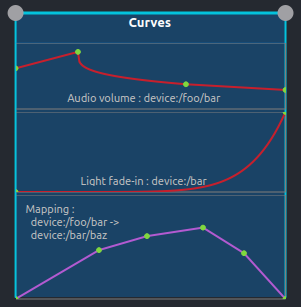
\includegraphics[scale=0.7]{images/curves.png}
        	\caption{Various kinds of curves}
        \end{figure}    
    \end{frame}
    
    \begin{lrbox}{\codebox}
    	\begin{lstlisting}
function(t) { 
    var obj = new Object; 
    obj["address"] = 'dev:/foo/bar'; 
    obj["value"] = t + iscore.value('other:/baz'); 
    return [ obj ]; 
}
    	\end{lstlisting}
    \end{lrbox}
    
    \begin{frame}
    	\frametitle{JavaScript}
    	\begin{figure}
    		\centering
    	    \usebox{\codebox}
    	    \caption{Will get called at each tick}
    	\end{figure}
    	
    	\begin{itemize}
    		\item Uses Qt's QJSEngine.
    		\item For now API with a single function : fetch a remote value.
    	\end{itemize}
    \end{frame}
    
    \begin{frame}
        \frametitle{Hierarchy}
        
        \begin{figure}
        	\centering
        	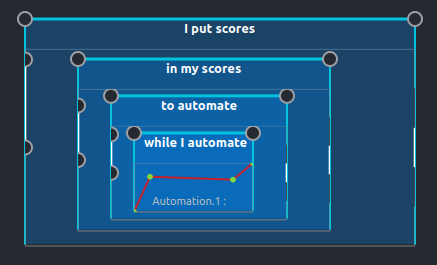
\includegraphics[scale=0.6]{images/hierarchy.png}
        	\caption{Scenarios can be \textbf{nested} arbitrarily}
        \end{figure}   
    \end{frame}
    
    \begin{frame}
        \frametitle{WIP : Spatial automations}
        
        \begin{figure}
        	\centering
        	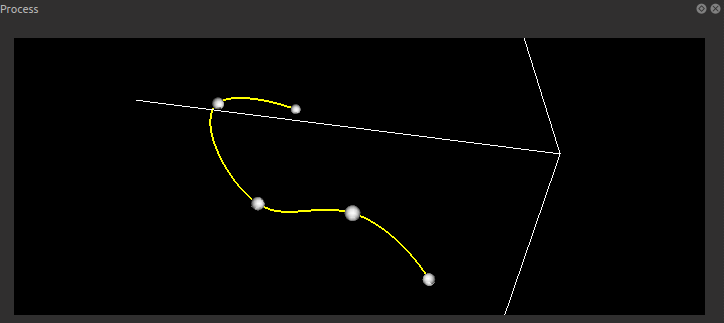
\includegraphics[width=\textwidth]{images/autom3d.png}
        \end{figure}   
        
        \begin{itemize}
        	\item \textbf{3d splines} that uses VTK. Can be used to create paths in space for instance.
        	\item \textbf{Spatial mappings} to compute collisions, distances, etc. and performs actions according to the result of such computations.
        \end{itemize}
    \end{frame}
    

\begin{frame}
    \frametitle{Future : distribution ?}
    
    \Large
    \begin{itemize}
        \setlength\itemsep{1em}
    	\item Currently : multiple instances can work together at the editing stage.
    	\item In progress : distributed execution.
    	\item Example scenarios :
    	\begin{itemize}
    		\item \large  100 phones controlling a parameter together.
    		\item Live backups if a computer dies during performance.
    		\item Offloading due to performance requirements.
    	\end{itemize}
    	 
    \end{itemize}
\end{frame}

\begin{frame}
    \frametitle{Future : other features}
    \Large
    \begin{itemize}
        \setlength\itemsep{1em}
    \item \textbf{MIDI}, \textbf{WebSockets} support
    \item Some level of \textbf{patching}, like Pd
    \item Complete \textbf{remote-control} abilities.\\ Currently : execution can be followed via a web page.
    \item Port execution engine to \textbf{FPGA}. 
    \item Audio engine ? 
    \end{itemize}
\end{frame}

\begin{frame}
    \frametitle{Contributing}   
    \large 
    \begin{itemize}
        \setlength\itemsep{1em}
    \item \textbf{UX}, \textbf{UI} (mock-ups were done but not entirely implemented)
    \item \textbf{Documentation}, writing demo scenarios
    \item \textbf{Translations}    
    \item Implement the \textbf{Minuit} protocol in your software with the OSSIA API    
    \item Many "low-hanging fruit" TODOs
    \item Mobile devices ports : 
    \begin{itemize}
        \item \textbf{Android} : builds and run but requires adapted UI.
        \item \textbf{Web port} : with PNaCl, runs but crashes. Will open the way to WebAssembly. 
        \item \textbf{iDevices} (many artists use them).
    \end{itemize}
\end{itemize}
    
\end{frame}



\begin{frame}
    \frametitle{Links}
    \begin{itemize}
        \setlength\itemsep{1em}
        \item \textbf{Grab a release !} ~\\ \url{github.com/OSSIA/i-score/releases}
        \item \textbf{Protocols and implementations} :~\\
        \url{github.com/OSSIA}
         \item \textbf{Official website (not up-to-date)} :~\\
         \url{i-score.org}
    \end{itemize}
        
    \centering
    \vspace{2em}
    \Large{Thanks ! Questions ?}
    \vspace{2em}
    
    \small{Credits: 'simple' Beamer theme, Facundo Muñoz; Fira font}
\end{frame}    
\end{document}
